%% SpecDx: manuscript for ACM Transactions on Software Engineering and Methodology (TOSEM).
%% Build: latexmk -pdf main.tex
% T5 is loaded alongside T1 so that Vietnamese words from the subject can be typeset.
\PassOptionsToPackage{T5,T1}{fontenc}
\documentclass[acmsmall,screen,review,anonymous]{acmart}

\usepackage{mathtools} % acmart already loads amsmath, amsthm and newtxmath (which provides the AMS symbols)
\usepackage{booktabs,multirow,makecell}
\usepackage{tikz}
\usetikzlibrary{arrows.meta,positioning,fit,calc,backgrounds,shapes.geometric,patterns,decorations.pathreplacing}
\usepackage{pgfplots}
\pgfplotsset{compat=1.18}
\usepgfplotslibrary{groupplots,colormaps}
\usepackage{algorithm}
\usepackage{algpseudocode}
\usepackage{subcaption}
\usepackage{enumitem}
\usepackage{xspace}
\usepackage[capitalise,nameinlink]{cleveref}

%% Notation shared by every section.
\newcommand{\specdx}{\textsc{SpecDx}\xspace}
\newcommand{\Tell}{\mathcal{T}}
\newcommand{\Chk}{\mathcal{C}}
\newcommand{\Scen}{\Pi}
\newcommand{\Spec}{\mathcal{S}}
\newcommand{\Beh}{\mathcal{B}}
\newcommand{\Adm}{\mathrm{Adm}}
\newcommand{\Models}{\mathcal{M}}
\newcommand{\Cells}{\mathcal{K}}
\newcommand{\Sets}{\mathfrak{A}}
\newcommand{\Pop}{\mathcal{I}}
\newcommand{\sig}{\sigma}
\newcommand{\one}{\mathbb{1}}
\newcommand{\E}{\mathbb{E}}
\newcommand{\Prob}{\mathbb{P}}
\newcommand{\Dir}{\mathrm{Dir}}
\newcommand{\Norm}{\mathcal{N}}
\newcommand{\other}{\textsc{other}}
\newcommand{\sat}{\textsf{sat}}
\newcommand{\viol}{\textsf{viol}}
\newcommand{\na}{\textsf{n/a}}
\newcommand{\KL}{\mathrm{KL}}
\newcommand{\logit}{\operatorname{logit}}
\newcommand{\median}{\operatorname*{median}}
\newcommand{\argmax}{\operatorname*{arg\,max}}
\newcommand{\argmin}{\operatorname*{arg\,min}}
\newcommand{\defeq}{\coloneqq}

%% Placeholder for numbers that the experiments have not produced yet.
\newcommand{\tbd}{\textcolor{gray}{--}}
\newcommand{\tbdnum}{\textcolor{gray}{[\,--\,]}}

%% acmart already defines theorem, lemma, proposition, corollary and definition.
\theoremstyle{remark}
\newtheorem*{remark}{Remark}

%% Short names for the four defect types.
\newcommand{\Dcon}{\textsc{Contradiction}\xspace}
\newcommand{\Dhid}{\textsc{Hidden}\xspace}
\newcommand{\Damb}{\textsc{Ambiguity}\xspace}
\newcommand{\Dweak}{\textsc{Weak}\xspace}

\newcommand{\rqref}[1]{\textbf{RQ#1}}

%% A boxed answer at the end of each research question.
\newcommand{\rqanswer}[2]{\par\smallskip\noindent\fbox{\parbox{\dimexpr\linewidth-2\fboxsep-2\fboxrule\relax}{\textbf{Answer to RQ#1.} #2}}\par\smallskip}
%% A type the method does not report.
\newcommand{\nr}{\textcolor{gray}{n/r}}

%% Vietnamese text from the subject (Latin Modern in T5 encoding; the main font has no T5).
\newcommand{\vi}[1]{{\fontencoding{T5}\fontfamily{lmr}\selectfont #1}}
%% Vietnamese status values used inside TikZ loops (robust, so \foreach does not expand them).
\DeclareRobustCommand{\viDa}{\vi{Đã duyệt}}
\DeclareRobustCommand{\viCho}{\vi{Chờ duyệt}}


\setcopyright{none}
\acmJournal{TOSEM}
\acmVolume{0}
\acmNumber{0}
\acmArticle{0}
\acmYear{2026}
\acmMonth{10}

\begin{document}

\title[When the Specification Is the Bug]{When the Specification Is the Bug: Diagnosing Executable Business Specifications with Populations of LLM Interpreters}

\author{Anonymous Author(s)}
\affiliation{%
  \institution{Anonymous Institution}
  \country{Anonymous Country}}

\begin{abstract}
Business automation and agent benchmarks increasingly rely on \emph{executable specifications}. Such a specification pairs natural-language requirements and policies, which tell an executor what to do, with executable checks that decide whether the result is right. These checks are usually treated as ground truth, yet recent audits of widely used agent benchmarks show that they are often wrong: they demand outcomes the requirements never state, accept behaviours the requirements forbid, or contradict each other. Finding such defects is hard. Static review of the text never sees the system run. Purely statistical audits cannot tell a bad specification from a weak model. Purely symbolic analysis of the checks cannot see the requirements at all.

We present \specdx, an automatic method that diagnoses executable specifications by running them with a population of local, open-weight LLM interpreters drawn from several model families. Each run is treated as one sample of how a reasonable executor reads the requirements. The core of \specdx is an \emph{anchored cell model}: a latent-class model in which the specification itself is one fallible rater, each checked value has a latent \emph{set} of admissible readings, and each interpreter has an accuracy that depends on its ability and on the difficulty of what it reads. We prove that, under stated assumptions, the defect form of each cell is identifiable from how its readings change with interpreter accuracy, and we give finite-sample bounds. \specdx combines this statistical evidence with logic. It enumerates minimal unsatisfiable subsets from the runs' violation sets and refutes candidates with witness states, localises ambiguities to sentences of the requirements by delta debugging, and chooses informative scenarios by Thompson sampling. It reports four typed defects: contradictions, hidden requirements, ambiguities and weak checks.

We evaluate \specdx on a procure-to-pay specification with seeded and real defects, under a pre-registered protocol. It is compared with seven published baselines that run on the same specifications, models, runs and scoring. [Results to be added: typed F1, real-defect recall and cost-effectiveness.]

\end{abstract}

\begin{CCSXML}
<ccs2012>
<concept>
<concept_id>10011007.10011074.10011099.10011102.10011103</concept_id>
<concept_desc>Software and its engineering~Software testing and debugging</concept_desc>
<concept_significance>500</concept_significance>
</concept>
<concept>
<concept_id>10011007.10011074.10011075.10011076</concept_id>
<concept_desc>Software and its engineering~Requirements analysis</concept_desc>
<concept_significance>500</concept_significance>
</concept>
<concept>
<concept_id>10002950.10003648.10003662</concept_id>
<concept_desc>Mathematics of computing~Probabilistic inference problems</concept_desc>
<concept_significance>300</concept_significance>
</concept>
</ccs2012>
\end{CCSXML}
\ccsdesc[500]{Software and its engineering~Software testing and debugging}
\ccsdesc[500]{Software and its engineering~Requirements analysis}
\ccsdesc[300]{Mathematics of computing~Probabilistic inference problems}

\keywords{specification defects, executable specifications, test oracles, large language models, latent class models, truth inference, minimal unsatisfiable subsets, benchmark validity}

\maketitle

\section{Introduction}
\label{sec:intro}

\subsection{Executable specifications are trusted, and wrong}

A growing share of software is judged by specifications that can be executed. A business process for an LLM agent comes with natural-language procedures and policies that tell the agent what to do. It also comes with database invariants, expected outcomes and guardrails that decide whether the agent did it right~\cite{calvanese2026agentic,li2025sopbench,levy2026webagentbench}. Agent benchmarks follow the same pattern:
\begin{itemize}[leftmargin=*]
\item $\tau$-bench and $\tau^2$-bench give agents a domain policy and score them against an expected database state~\cite{yao2025bench,barres2026bench};
\item SWE-bench scores patches with the project's own tests~\cite{jimenez2024swe}.
\end{itemize}
We call such an artefact an \emph{executable business specification}. It has two parts that must agree: a \emph{Tell} part $\Tell$, which is everything an executor is told, and a \emph{Check} part $\Chk$, which is everything a result is judged by. The systems and studies built on these specifications treat $\Chk$ as ground truth.

That trust is often misplaced. Audits of the most widely used agent benchmarks keep finding checks that are wrong:
\begin{itemize}[leftmargin=*]
\item Cuadron et al.\ traced ceiling effects in $\tau$-bench to annotation errors and underspecified tasks, and released a verified version with targeted repairs~\cite{cuadron2025saber}.
\item A systematic checklist study found, among other flaws, that $\tau$-bench counted some empty responses as successes~\cite{zhu2025establishing}.
\item Many SWE-bench patches that pass the tests are still wrong~\cite{wang2026solved,yu2025utboost,yu2026swe}. The tests of popular code benchmarks miss many wrong programs~\cite{liu2023your}.
\item Expert audits report ground truths that are incorrect, underspecified or contradictory across agent, coding and data-engineering benchmarks~\cite{zanoli2026elt,bhat2026benchmarking,wang2026automated,cao2026policy}.
\end{itemize}
The same problem appears outside benchmarks. Label errors destabilise machine-learning test sets~\cite{northcutt2021pervasive,gema2025done}, and even formally verified systems fail because their specifications are wrong~\cite{fonseca2017empirical}. When the specification is the bug, an agent that does the right thing is scored as wrong, and conclusions about which system is better can flip~\cite{northcutt2021pervasive,cao2026policy}.

\subsection{Why the defects are hard to find}

A specification defect is a disagreement between $\Tell$ and $\Chk$, or inside $\Chk$. We distinguish four kinds:
\begin{itemize}[leftmargin=*]
\item a \emph{contradiction}: no behaviour can satisfy the checks;
\item a \emph{hidden requirement}: the checks demand something the text does not say;
\item an \emph{ambiguity}: the text allows more than one reading;
\item a \emph{weak check}: a behaviour the text forbids still passes every check.
\end{itemize}
Current approaches see only part of this picture.

\paragraph{Static review reads, but never runs.} Work on requirements quality detects ambiguity, incompleteness and inconsistency in natural-language text~\cite{berry2003contract,chantree2006identifying,femmer2017rapid,gervasi2005reasoning}. Recent work does so with LLMs~\cite{fantechi2023inconsistency,gartner2024automated,hall2026neurosymbolic}. LLM auditors now review benchmark tasks, graders and reference solutions automatically~\cite{tu2026who,wang2026automated,suh2026agentsuite,mohl2026automated}. These tools read the artefacts. They do not observe what a reasonable executor actually does when it follows the text, so they cannot see where executions and checks part ways. They also rely on a single auditor's judgement.

\paragraph{Population statistics see disagreement, but not its cause.} A second line of work learns from the answers of many models.
\begin{itemize}[leftmargin=*]
\item Item response theory flags benchmark items whose difficulty profile looks wrong~\cite{rodriguez2021evaluation,land2026auditing}.
\item Confident learning and LLM ensembles flag likely label errors~\cite{northcutt2021confident,nahum2025llms,klie2023annotation}.
\item Disagreement and semantic entropy flag uncertain inputs~\cite{kuhn2023semantic,farquhar2024detecting,zhang2025stress}.
\end{itemize}
These methods assume one correct answer per item, so they cannot express an item that has two correct answers or none. They cannot say which kind of defect they found or where it sits in the text. They also struggle with a well-documented fact: errors of different LLMs are correlated~\cite{kim2025correlated,goel2025great}, and models faced with an underspecified prompt tend to collapse onto a single reading instead of exposing the alternatives~\cite{richter2026underspecification}. Raw disagreement is therefore a weak signal.

\paragraph{Symbolic analysis sees the checks, but not the text.} Minimal unsatisfiable subsets and unsatisfiable cores find conflicts inside a set of constraints~\cite{liffiton2008algorithms,torlak2008finding,shlyakhter2003debugging}. Vacuity detection and oracle assessment find checks that are too loose~\cite{kupferman2003vacuity,jahangirova2016test,schuler2011assessing}. All of these work on $\Chk$ alone, so they cannot tell that a check demands something $\Tell$ never says.

The closest existing work combines execution with disagreement:
\begin{itemize}[leftmargin=*]
\item ClarifyGPT and SpecFix call a requirement ambiguous when programs sampled from one model disagree~\cite{mu2024clarifygpt,jia2025automated}.
\item JEST runs several JavaScript engines and blames the specification when most of them fail the same test~\cite{park2021jest}.
\end{itemize}
These methods either trust the checks, use a single model with no notion of its competence, or assume near-deterministic executors. None of them types its findings or backs them with logical witnesses.

\subsection{Our approach}

Our starting point is simple. An LLM agent that executes a specification is a fallible but cheap \emph{reasonable reader}. One run tells us little, because the agent may simply be wrong. Many runs from several model families, each reading the same text under paraphrase and sampling noise, tell us how reasonable readers interpret it. The evidence then sorts itself as follows:
\begin{itemize}[leftmargin=*]
\item If competent readers agree with each other but not with $\Chk$, the check is suspect.
\item If they split into stable camps, the text is ambiguous.
\item If a run that the population considers wrong still passes every check, a check is weak.
\item If no run, however competent, satisfies a set of clauses together, the clauses may contradict each other.
\end{itemize}

Turning this intuition into a method requires answers to three questions:
\begin{itemize}[leftmargin=*]
\item[\textbf{Q1.}] How can we separate interpreter error from specification defect, when models differ in competence and the ``truth'' of a check may be a set of values or no value at all?
\item[\textbf{Q2.}] How can we turn noisy evidence into findings that are typed, located and backed by witnesses?
\item[\textbf{Q3.}] How should a limited budget of runs be spent?
\end{itemize}

We answer them with \specdx.
\begin{itemize}[leftmargin=*]
\item \textbf{Q1: the anchored cell model.} For Q1, \specdx reads every run cell by cell, where a cell is one checked value or one clause. It fits an \emph{anchored cell model}, a latent-class model in the tradition of Dawid and Skene~\cite{dawid1979maximum} and GLAD~\cite{whitehill2009whose}, with three changes:
  \begin{itemize}
  \item the specification's declared value is an anchor, so the specification is one more fallible rater;
  \item the latent truth of a cell is a \emph{set} of admissible readings, which may hold one value, two values or none;
  \item an interpreter's accuracy depends on its ability and on the cell's difficulty, and its errors never fall on an admissible value.
  \end{itemize}
  We prove that under these assumptions each defect form leaves a distinct \emph{accuracy-gradient signature}, and that the forms are identifiable with finite-sample guarantees.
\item \textbf{Q2: combining statistics with logic.} Each run's set of violated clauses is a sampled correction set, so minimal hitting sets of these sets give candidate minimal unsatisfiable subsets~\cite{reiter1987theory,liffiton2008algorithms}. Every candidate is then put to a refutation step that searches for a witness state. Ambiguities are localised to sentences of $\Tell$ by delta debugging~\cite{zeller2002simplifying}.
\item \textbf{Q3: active scenario choice.} \specdx chooses the next scenario by Thompson sampling~\cite{russo2018tutorial}, using boundary values taken from the text. It runs a cheap pilot of one model per family before committing the full population.
\end{itemize}

We evaluate \specdx on a Vietnamese procure-to-pay specification from the TonomyX project. The specification has nine gated tools, a 26-table database and three requirement documents. We seed 36 defects with nine mutation operators and also study defects recorded in the project's history. The study is pre-registered: every threshold is chosen by simulation or on base data before any seeded defect is seen. \specdx is compared with seven published baselines and two secondary arms, all run on the same specifications, models, cached runs and scoring code. [Summary of the results to be added once the experiments are complete.]

\subsection{Contributions}

\begin{enumerate}[leftmargin=*,label=\textbf{C\arabic*.}]
\item \textbf{A formal model of executable business specifications.} We define the specification as $\Spec=\langle\Tell,\Chk,\Scen\rangle$, a four-type defect taxonomy defined purely by satisfaction, and a cell-level view of behaviours that lifts checks across scenarios (\cref{sec:problem}).
\item \textbf{The anchored cell model.} This is a latent-class model with set-valued truth, anchors, item difficulty and a restricted error distribution, fitted by penalised EM (\cref{sec:approach}).
\item \textbf{Identifiability results.} We give accuracy-gradient signatures, identification of every defect form from two models with different accuracies or from one model with a known error pool, identification of model contrasts from anchors with a breakdown point of one half, and Hoeffding-type finite-sample bounds (\cref{sec:theory}).
\item \textbf{Typed, witnessed diagnosis.} We combine the cell posteriors with hitting sets over sampled correction sets, sound refutation, delta-debugging localisation in the text, and active scenario synthesis with sequential escalation (\cref{sec:approach}).
\item \textbf{An evaluation framework and study.} We provide specification mutation operators with kill witnesses, observability-aware scoring, a pre-registered gate, and a fair comparison protocol against seven baselines with frozen, development-only choices. The empirical study and an open artefact complete the contribution (\cref{sec:eval-design,sec:results}).
\end{enumerate}

\paragraph{Organisation.}
\begin{itemize}[leftmargin=*]
\item \Cref{sec:motivating} walks through a real defect.
\item \Cref{sec:problem} formalises the problem, \cref{sec:approach} presents \specdx and \cref{sec:theory} its theory.
\item \Cref{sec:eval-design,sec:results} describe the evaluation and its results.
\item \Cref{sec:discussion,sec:threats} discuss implications and threats to validity.
\item \Cref{sec:related} relates \specdx to prior work and \cref{sec:conclusion} concludes.
\end{itemize}

\section{Motivating Example}
\label{sec:motivating}

We illustrate the problem with two defects recorded in the history of TonomyX, an open platform in which ``digital employees'' (LLM agents with scoped tools) carry out a Vietnamese procure-to-pay process under human approval gates. Its reference case, CASE-0031, follows one purchase from the sales order to payment:
\begin{itemize}[leftmargin=*]
\item a sales order (\texttt{SO-0031}) is created;
\item a purchase order (\texttt{PO-0015}) for 15 units is issued;
\item a goods receipt records 12 units;
\item a three-way match reconciles the order, the receipt and the invoice;
\item a payment is made.
\end{itemize}

The specification has the two parts introduced above:
\begin{itemize}[leftmargin=*]
\item \textbf{Tell, $\Tell$.} About 160 pages of requirements: a business-analysis document, a demo description and a software architecture document. To these come three knowledge-base articles and a list of business principles.
\item \textbf{Check, $\Chk$.} Forty-two database invariants, scenario expectations, a golden end state over 26 tables, guardrail triggers and a scope table that grants each digital employee its tools.
\end{itemize}
Both parts were written carefully by the same team, and the checks pass on the reference run. Yet both of the following defects went unnoticed for some time.

\paragraph{R-SO: a status the text never asks for.}
A human approver signs approval \texttt{APR-0102}. In the golden end state, the purchase order then moves to \emph{\vi{Đã duyệt}} (``approved''), while the sales order \texttt{SO-0031} stays at \emph{\vi{Chờ duyệt}} (``awaiting approval''). Nothing in $\Tell$ says that the sales order should stay pending once its approval is granted. An agent that carries out the approval and moves both documents forward is therefore doing what the text allows, but it violates the golden clause on \texttt{SO-0031} and is scored as failing. In our terms, $\Chk$ is stricter than $\Tell$ at one clause: a \emph{hidden requirement}.

\paragraph{R-12: a conflict that only shows off the beaten path.}
The database schema allows a purchase order to have several goods receipts, and the requirements describe partial deliveries. The reconciliation function \texttt{fn\_reconcile}, however, raises a cardinality error whenever a purchase order has more than one receipt. One invariant demands that the stored reconciliation result equal the value of \texttt{fn\_reconcile}. In any scenario with two receipts, no end state can satisfy that invariant together with the schema and the expectations: the clauses form a \emph{contradiction}. None of the three reference scenarios has two receipts, so the conflict stays invisible until someone tries one.

\paragraph{What existing approaches see.}
\Cref{tab:motivating} summarises what each family of methods can conclude on these two defects. The point is not that existing methods are weak, but that each one sees a different slice of the evidence.
\begin{itemize}[leftmargin=*]
\item \textbf{A static LLM reviewer} reads $\Tell$ and $\Chk$ side by side. Finding R-SO requires it to notice the absence of a rule across 160 pages. Finding R-12 requires it to reason about the behaviour of a SQL function in a scenario that nobody wrote down.
\item \textbf{A single agent run} that violates the clause on \texttt{SO-0031} looks like any other agent failure. Failure-attribution methods~\cite{zhang2025which} would most likely blame the agent.
\item \textbf{Population statistics} would see that many runs violate the clause. They could not tell a hidden requirement from a clause that is simply hard to satisfy, or from an ambiguity in which the population splits.
\item \textbf{A MUS solver over $\Chk$ alone} cannot find R-SO at all, because the golden clause is consistent with the other checks. It can find R-12 only if \texttt{fn\_reconcile} is encoded, and only if it explores a scenario with two receipts.
\end{itemize}

\begin{table}[t]
\caption{What each family of methods can conclude on the two motivating defects. The entries are qualitative, not measured: they follow from what each method observes.}
\label{tab:motivating}
\small
\begin{tabular}{@{}p{3.2cm}p{4.9cm}p{4.9cm}@{}}
\toprule
Method family & R-SO (hidden requirement) & R-12 (contradiction) \\
\midrule
Static LLM review of $\Tell$ and $\Chk$ & Must notice that a rule is \emph{absent} from a long text & Must simulate a SQL function in an unwritten scenario \\
Failure attribution on one run & Likely blames the agent & Sees an error, not its cause \\
Population statistics & Flags the clause, but cannot type it & Flags several clauses, without a conflict set \\
MUS over $\Chk$ alone & Cannot see it (the checks are consistent) & Finds it only if the function is encoded and the scenario is explored \\
\specdx (this paper) & Competent readers agree with each other, not with the anchor; refutation finds a state satisfying all other clauses $\Rightarrow$ \Dhid & Synthesised scenario with two receipts; no run or repair satisfies the conflict set $\Rightarrow$ \Dcon \\
\bottomrule
\end{tabular}
\end{table}

\paragraph{What \specdx does.}
\specdx runs the process many times with a population of local LLM interpreters, each reading the same $\Tell$ under paraphrase and seeds. On R-SO, it looks at one \emph{cell}: the status of \texttt{SO-0031} after the approval step. The specification declares \emph{\vi{Chờ duyệt}}, and this is the cell's anchor. If interpreters that are accurate elsewhere, on cells whose anchors they reproduce, read the cell as \emph{\vi{Đã duyệt}}, and if this reading becomes \emph{more} frequent as interpreter accuracy rises, then the anchor is the odd one out. The anchored cell model (\cref{sec:approach-model}) turns this pattern into a posterior probability that the anchor lies outside the set of readings $\Tell$ admits. A refutation step then confirms the type: it searches for an end state that satisfies every other clause, and finding one shows that the defect is a hidden requirement, not a contradiction.

On R-12, \specdx extracts the literals of $\Tell$ that bound its scenario parameters and adds boundary scenarios. It then lets Thompson sampling pick scenarios whose outcomes are uncertain, among them one with two receipts. Every run in that scenario violates some clause, and the minimal hitting sets of the violation sets point to the reconciliation clause. Because no repair of the state satisfies it, the finding is reported as a contradiction, with the failed refutation attempts as evidence.

\section{Problem Formulation}
\label{sec:problem}

This section fixes the vocabulary used in the rest of the paper. \Cref{tab:notation} lists the main symbols.

\subsection{Executable business specifications}

\begin{definition}[Executable business specification]
\label{def:spec}
An \emph{executable business specification} is a triple $\Spec=\langle\Tell,\Chk,\Scen\rangle$, where:
\begin{itemize}[leftmargin=*]
\item $\Tell$, the \emph{Tell} part, is everything an executor is told. In our subject these are the requirement documents, knowledge-base articles, business principles, tool catalogue, database schema, scope table and the refusal messages returned by tools.
\item $\Chk=\{\varphi_1,\dots,\varphi_{|\Chk|}\}$, the \emph{Check} part, is a finite set of clauses that can be evaluated on a behaviour. These are invariants, expectations, golden-state values, guardrails, blank-column rules and event vocabulary.
\item $\Scen$ is the scenario space. A scenario $\pi\in\Scen$ is a vector of task parameters, such as the ordered quantity, the received quantity, the requested discount and the number of receipts per order.
\end{itemize}
\end{definition}

We deliberately exclude any hand-written ``playbook'' that explains how to carry out the process. A playbook is one human's interpretation of $\Tell$. Including it would test the playbook, not the specification.

\paragraph{Behaviours.} A run of an executor on scenario $\pi$ produces a \emph{behaviour} $b$. It consists of the rows the run committed to the database, the events it logged, the tool calls the guardrails refused and the executor's final claim. Each clause is a function
\begin{equation}
\label{eq:eval}
\varphi:\Beh\to\{\sat,\viol,\na\},
\end{equation}
where $\na$ means that the clause does not apply, for instance because the rows it reads do not exist in $b$. We write $b\models\varphi$ when $\varphi(b)=\sat$, and $b\models\Chk'$ when $b\models\varphi$ for every applicable $\varphi\in\Chk'$. The \emph{violation set} of $b$ is
\begin{equation}
\label{eq:violset}
V(b)=\{\varphi\in\Chk:\varphi(b)=\viol\}.
\end{equation}

\paragraph{Clause lifting.} Many clauses state facts of one reference case as literals, such as ``the ordered quantity equals 15''. \emph{Lifting} rewrites such a clause into a form that depends on the scenario, here $\textit{ordered}=\pi.\textit{ordered}$. It does so by anti-unifying the clause's literals with the parameters of the reference scenarios. A literal is lifted only when it matches the same parameter in every reference scenario; otherwise the clause stays bound to the scenario it came from. We write $\Chk(\pi)$ for the lifted clauses that apply in $\pi$.

\paragraph{Specification-induced equivalence.} Two behaviours may differ in ways the specification does not care about, such as timestamps, serial identifiers or free text. The relation $\equiv_\Spec$ compares behaviours only on the \emph{locked} columns: keys, statuses, quantities, approvals and the $(\textit{kind},\textit{ref},\textit{actor})$ of events. It also requires the \emph{blank} columns to be null in both behaviours. The classification of every column is derived automatically from the schema and the specification's metadata, so the specification itself, and not the researcher, decides what counts as ``the same outcome''.

\subsection{Interpreters and admissible behaviours}

An \emph{interpreter} $I$ maps $(\Tell,\pi)$ to a behaviour at random. An interpreter is a model $m$ together with a Tell variant $v$ and a sampling seed $r$. The ideal interpreter $I^\star$ produces exactly the behaviours that $\Tell$ permits,
\begin{equation}
\label{eq:adm}
\Adm_\Tell(\pi)\subseteq\Beh .
\end{equation}
$\Adm_\Tell(\pi)$ is never observed directly; it is the object that \specdx estimates. A population $\Pop=\{(m,v,r)\}$ draws from $\Models\times\{0,1,2\}\times\{1,2,3\}$. Variant 0 is the original text. Variants 1 and 2 paraphrase only the standing instruction and the task statement, so that a seeded ambiguity in the retrieved requirements is not washed out.

\subsection{Defect taxonomy}

Each defect type is defined purely by satisfaction on a scenario $\pi$.

\begin{definition}[Defect types]
\label{def:defects}
Let $\pi\in\Scen$.
\begin{enumerate}[leftmargin=*,label=(\roman*)]
\item \textbf{Contradiction.} A set $M\subseteq\Chk(\pi)$ is a contradiction when no behaviour satisfies it:
  \begin{equation}\label{eq:def-con}
  \nexists\,b\in\Beh:\;b\models M .
  \end{equation}
  It is reported as a minimal unsatisfiable subset (MUS).
\item \textbf{Hidden requirement.} A clause $\varphi$ is a hidden requirement when some admissible behaviour satisfies every other clause but not $\varphi$:
  \begin{equation}\label{eq:def-hid}
  \exists\,b\in\Adm_\Tell(\pi):\;b\models\Chk(\pi)\setminus\{\varphi\}\;\wedge\;b\not\models\varphi .
  \end{equation}
  Here $\Chk$ is stricter than $\Tell$ at $\varphi$.
\item \textbf{Ambiguity.} $\Tell$ is ambiguous at $\pi$ when it admits more than one outcome up to $\equiv_\Spec$:
  \begin{equation}\label{eq:def-amb}
  \bigl|\Adm_\Tell(\pi)/{\equiv_\Spec}\bigr|\ge 2 .
  \end{equation}
  It is located at the sentences of $\Tell$ responsible for the split.
\item \textbf{Weak check.} $\Chk$ is weak at $\pi$ when a behaviour that $\Tell$ forbids passes every check:
  \begin{equation}\label{eq:def-weak}
  \exists\,b\notin\Adm_\Tell(\pi):\;b\models\Chk(\pi) .
  \end{equation}
  Here $\Chk$ is looser than $\Tell$. The defect is located at the locked field on which $b$ departs from the admissible outcomes.
\end{enumerate}
\end{definition}

\Cref{fig:taxonomy} pictures the four definitions as relations between two sets of behaviours: those that $\Tell$ admits and those that pass the checks.

\begin{figure}[t]
\centering
\resizebox{\textwidth}{!}{% Defect taxonomy as relations between the admissible behaviours and the behaviours that pass the checks.
\begin{tikzpicture}[
  every node/.style={font=\footnotesize},
  adm/.style={draw=blue!60!black, fill=blue!12, fill opacity=0.8, text opacity=1},
  sat/.style={draw=orange!80!black, fill=orange!18, fill opacity=0.65, text opacity=1},
  beh/.style={draw=gray, rounded corners=2pt},
  pt/.style={circle, fill=black, inner sep=1.3pt}]
\foreach \x/\t in {0/{(a) Contradiction}, 3.55/{(b) Hidden requirement}, 7.1/{(c) Ambiguity}, 10.65/{(d) Weak check}} {
  \draw[beh] (\x,0) rectangle ++(3.25,2.6);
  \node[anchor=north west, gray] at (\x,2.6) {$\Beh$};
  \node[anchor=north, font=\footnotesize\bfseries] at (\x+1.625,-0.05) {\t};
}
% (a) no behaviour satisfies M
\draw[adm] (0.95,1.35) ellipse (0.7 and 0.55); \node at (0.95,1.35) {$\Adm_\Tell$};
\draw[draw=red!70!black, dashed, thick] (2.45,1.5) circle (0.4);
\draw[red!70!black, thick] (2.17,1.22) -- (2.73,1.78) (2.17,1.78) -- (2.73,1.22);
\node[red!70!black, align=center, font=\scriptsize] at (1.85,0.4) {no $b$ with $b\models M$};
% (b) an admissible behaviour fails one clause
\begin{scope}[shift={(3.55,0)}]
\draw[sat] (2.0,1.3) ellipse (1.05 and 0.8); \node at (2.45,1.75) {$\textsf{Sat}(\Chk)$};
\draw[adm] (1.05,1.2) ellipse (0.8 and 0.6); \node at (0.95,1.45) {$\Adm_\Tell$};
\node[pt] (b) at (0.6,1.0) {}; \node[font=\scriptsize, align=center] at (1.62,0.3) {$b\models\Chk\setminus\{\varphi\}$, $b\not\models\varphi$};
\end{scope}
% (c) two admissible classes
\begin{scope}[shift={(7.1,0)}]
\draw[adm] (1.62,1.3) ellipse (1.25 and 0.75);
\draw[blue!60!black, dashed] (1.62,0.55) -- (1.62,2.05);
\node at (1.05,1.3) {$[b_1]$}; \node at (2.2,1.3) {$[b_2]$};
\node[font=\scriptsize] at (1.62,0.3) {$|\Adm_\Tell/{\equiv_\Spec}|\ge2$};
\end{scope}
% (d) a non-admissible behaviour passes every check
\begin{scope}[shift={(10.65,0)}]
\draw[sat] (1.62,1.4) ellipse (1.3 and 0.85); \node at (2.35,1.95) {$\textsf{Sat}(\Chk)$};
\draw[adm] (1.25,1.25) ellipse (0.65 and 0.45); \node at (1.25,1.25) {$\Adm_\Tell$};
\node[pt] at (2.45,0.95) {}; \node[font=\scriptsize] at (1.62,0.22) {$b\notin\Adm_\Tell$, $b\models\Chk$};
\end{scope}
\end{tikzpicture}
}
\caption{The four defect types as relations between the admissible behaviours $\Adm_\Tell$ and the behaviours that pass the checks, $\textsf{Sat}(\Chk)$, inside the space of behaviours $\Beh$. (a)~No behaviour satisfies a clause set $M$. (b)~An admissible behaviour fails exactly one clause. (c)~The admissible behaviours fall into two classes of $\equiv_\Spec$. (d)~A behaviour outside $\Adm_\Tell$ passes every check.}
\label{fig:taxonomy}
\end{figure}

The types may co-occur. When $\Tell$ is ambiguous and $\Chk$ picks one of the readings, both an ambiguity and a hidden requirement are reported: the behaviours that follow the other reading satisfy \eqref{eq:def-hid}.

The definitions show why no single source of evidence is enough. A contradiction~\eqref{eq:def-con} concerns $\Chk$ alone. Sampling can never prove that no behaviour exists, so a contradiction can only be supported by failed attempts and refuted by a witness. A hidden requirement~\eqref{eq:def-hid} and an ambiguity~\eqref{eq:def-amb} quantify over $\Adm_\Tell$, which only an interpreter of $\Tell$ can sample. A weak check~\eqref{eq:def-weak} quantifies over behaviours \emph{outside} $\Adm_\Tell$, which an ideal interpreter never produces. Its detection therefore relies on interpreters that err. The following proposition makes the role of ideal interpreters precise.

\begin{proposition}[Soundness under ideal interpreters]
\label{prop:ideal}
Suppose every observed behaviour on $\pi$ is drawn from $\Adm_\Tell(\pi)$.
\begin{enumerate}[leftmargin=*,label=(\alph*)]
\item If an observed $b$ has $V(b)=\{\varphi\}$, then $\varphi$ is a hidden requirement. Whether $\varphi$ is also unsatisfiable on its own, a contradiction of size one, is left to refutation.
\item If two observed behaviours are not $\equiv_\Spec$-equivalent, then $\Tell$ is ambiguous at $\pi$.
\item If every clause is invariant under $\equiv_\Spec$ and the sample covers every class of $\Adm_\Tell(\pi)/{\equiv_\Spec}$, both tests are complete.
\end{enumerate}
\end{proposition}
The proof is in \cref{app:proofs}. Real interpreters are not ideal: they err, abstain, and err in correlated ways. The rest of the method is about recovering conclusions (a)--(c) when the observed behaviours mix admissible readings with interpreter errors.

\subsection{Cells: the unit of evidence}
\label{sec:cells}

Comparing whole behaviours is too coarse. Independent variation in several fields multiplies into many distinct outcomes, and nearly every pair of runs differs somewhere. \specdx therefore reads every behaviour at the level of \emph{cells}. We first define items.

\paragraph{Items.} An \emph{item} $s=(\pi,\textit{step})$ is one interpreter step of the process in a scenario.

\paragraph{Cells.} A \emph{cell} is the smallest unit of reading. There are two kinds.
\begin{itemize}[leftmargin=*]
\item A \emph{value cell} is a locked (table, row, column) triple, or one golden event $(\textit{kind},\textit{ref},\textit{actor})$. Its reading $y_{b,c}$ is the normalised value of the field in $b$'s end state, or \textsf{absent}.
\item A \emph{constraint cell} is one cross-cutting clause evaluated at an item. Its reading is $\sat$ or $\viol$.
\end{itemize}

\paragraph{Anchors.} The \emph{anchor} $d_c$ of a cell is what $\Chk$ declares for it: the (lifted) golden value of a value cell, \textsf{present} for a golden event, and $\sat$ for a constraint cell. A value cell on which $\Chk$ declares nothing is \emph{unanchored}. Unanchored cells contribute no evidence about accuracy, but they are where weak checks show up.

\paragraph{Pooling.} A lifted cell is one cell across all the scenarios where it applies. Its readings are pooled in the lifted vocabulary: a reading that equals the scenario's value of the parameter \textit{qty} is recorded as the placeholder \texttt{\{qty\}} in every scenario. Pooling increases the number of readings per cell, which the finite-sample bounds of \cref{sec:theory} depend on.

\Cref{fig:cells} shows what the data look like: a matrix of behaviours by cells, with the anchors in the first row and gaps where a behaviour did not act.

\begin{figure}[t]
\centering
\resizebox{0.95\textwidth}{!}{% From runs to cell readings: an illustrative reading matrix.
\begin{tikzpicture}[
  every node/.style={font=\footnotesize},
  cell/.style={draw=gray!60, minimum width=1.55cm, minimum height=0.5cm, inner sep=1pt},
  hd/.style={cell, fill=gray!10, font=\scriptsize, align=center, minimum height=0.85cm},
  an/.style={cell, fill=orange!18},
  miss/.style={cell, fill=gray!25, text=gray}]
\def\W{1.6}
% header
\node[anchor=east] at (-0.88,0.4) {cell $c$};
\foreach \i/\h in {0/{status of\\\texttt{SO-0031}}, 1/{\texttt{po.sl\_dat}\\(lifted)}, 2/{event \textsf{PAID}\\\texttt{PAY-0031}}, 3/{no declared\\value}, 4/{clause $\varphi$\\(constraint cell)}}
  \node[hd] at (\i*\W,0.4) {\h};
\node[anchor=east] at (-0.88,-0.35) {anchor $d_c$};
\foreach \i/\v in {0/{\viCho}, 1/{\texttt{\{qty\}}}, 2/{\textsf{present}}, 4/{\sat}}
  \node[an] at (\i*\W,-0.35) {\v};
\node[cell, fill=white, text=gray] at (3*\W,-0.35) {none};
% readings
\foreach \r/\lab/\va/\vb/\vc/\vd/\ve in {
  1/{$b_1$ (model 1)}/{\viDa}/{\texttt{\{qty\}}}/{\textsf{absent}}/{\texttt{0}}/{\sat},
  2/{$b_2$ (model 1)}/{\viCho}/{\texttt{\{qty\}}}/{\textsf{absent}}/{\texttt{0}}/{\viol},
  3/{$b_3$ (model 2)}/{\viDa}/{\texttt{12}}/{\textsf{absent}}/{\texttt{null}}/{\sat},
  4/{$b_4$ (model 3)}/{--}/{--}/{--}/{--}/{--},
  5/{$b_5$ (model 4)}/{\viDa}/{\texttt{\{qty\}}}/{\textsf{absent}}/{\texttt{0}}/{\sat}} {
  \node[anchor=east] at (-0.88,-0.35-0.55*\r) {\lab};
  \ifnum\r=4
    \foreach \i in {0,...,4} \node[miss] at (\i*\W,-0.35-0.55*\r) {no reading};
  \else
    \node[cell] at (0,-0.35-0.55*\r) {\va};
    \node[cell] at (\W,-0.35-0.55*\r) {\vb};
    \node[cell] at (2*\W,-0.35-0.55*\r) {\vc};
    \node[cell] at (3*\W,-0.35-0.55*\r) {\vd};
    \node[cell] at (4*\W,-0.35-0.55*\r) {\ve};
  \fi
}
% braces
\draw[decorate, decoration={brace, amplitude=4pt}] (-0.78,1.0) -- (3*\W+0.78,1.0) node[midway, above=4pt] {value cells (read from the end state)};
\draw[decorate, decoration={brace, amplitude=4pt}] (4*\W-0.78,1.0) -- (4*\W+0.78,1.0) node[midway, above=4pt, align=center] {constraint cell};
\node[anchor=west, align=left, font=\scriptsize, text width=3.0cm] at (4*\W+0.95,-1.95) {$b_4$ did not act at the item ($a_{bs}=0$): it contributes no reading, not a disagreement.};
\end{tikzpicture}
}
\caption{From runs to cell readings (illustrative values). Each row is one behaviour, each column one cell; the first row holds the anchors that $\Chk$ declares. Value cells are read from the end state, and a constraint cell is read as $\sat$ or $\viol$. A behaviour that did not act at the item contributes no reading.}
\label{fig:cells}
\end{figure}

The interpretation of a cell under each defect type follows from \cref{def:defects}. Let $A_c$ be the set of readings of $c$ that $\Tell$ admits. Then:
\begin{itemize}[leftmargin=*]
\item $A_c=\{d_c\}$ means no defect at $c$;
\item $d_c\notin A_c\neq\emptyset$ means a hidden requirement whose anchor is wrong (the \emph{mis-key} subtype);
\item $|A_c|=2$ means an ambiguity; when it contains $d_c$, $\Chk$ has picked one of the readings (the \emph{ambiguous-pick} subtype);
\item $A_c=\emptyset$ on an anchored cell means $\Tell$ says nothing about the cell while $\Chk$ fixes it (the \emph{unstated} subtype).
\end{itemize}
The subtypes are all hidden requirements in the sense of \eqref{eq:def-hid}, and they are reported as such.

\subsection{Problem statement}

\begin{quote}
\emph{Given} a specification $\Spec=\langle\Tell,\Chk,\Scen\rangle$, a population of local LLM interpreters $\Pop$ and a budget $B$ of runs, \emph{report} a ranked list of defects. Each defect carries a type from \cref{def:defects}, a location (a clause set, a clause, a set of sentences of $\Tell$, or a locked field), witness behaviours and a score. No human labels may be used.
\end{quote}

\begin{table}[t]
\caption{Main notation.}
\label{tab:notation}
\small
\begin{tabular}{@{}ll@{}}
\toprule
Symbol & Meaning \\
\midrule
$\Spec=\langle\Tell,\Chk,\Scen\rangle$ & Specification: Tell part, Check part (clauses $\varphi$), scenario space \\
$b$, $V(b)$ & Behaviour; its set of violated clauses \\
$\Adm_\Tell(\pi)$ & Behaviours that $\Tell$ permits in scenario $\pi$ \\
$m\in\Models$, $(m,v,r)\in\Pop$ & Model; interpreter (model, Tell variant, seed) \\
$s$, $a_{bs}$ & Item (scenario, step); act indicator \\
$\eta_m$, $\delta_s$, $O_s$ & Capability to act, item difficulty, observability (stage 1) \\
$c\in\Cells$, $d_c$, $V_c$ & Cell, its anchor, its candidate values (with \other) \\
$A_c\in\Sets_c$ & Latent set of admissible readings of $c$ \\
$\alpha_m$, $\beta_g$, $p_{m,c}$ & Model ability, group difficulty, accuracy $\sigma(\alpha_m-\beta_{g(c)})$ \\
$\varepsilon_c$, $\kappa$, $u_c$ & Error distribution, its concentration and flat pool \\
$r_{bc}$, $w_b$ & Probability that a reading is faithful; behaviour weight \\
$\tau_H,\tau_A,\tau_W$ & Typing thresholds (hidden, ambiguity, weak) \\
\bottomrule
\end{tabular}
\end{table}

\section{The \specdx Approach}
\label{sec:approach}

\Cref{fig:pipeline} gives an overview. \specdx works in rounds, and each round has five steps:
\begin{enumerate}[leftmargin=*]
\item It picks a scenario (\cref{sec:approach-scenarios}).
\item It runs a pilot of the population on that scenario, and the full population only if the pilot looks informative.
\item It reads each run at the level of items and cells (\cref{sec:approach-observe}).
\item It fits two statistical models: an act model that says where the evidence is reliable (\cref{sec:approach-act}), and the anchored cell model that says what $\Tell$ admits at each cell (\cref{sec:approach-model}).
\item It turns the posteriors into typed findings, which it backs with logical witnesses and localises in $\Tell$ (\cref{sec:approach-typing,sec:approach-localise}).
\end{enumerate}
The loop is \emph{anytime}: stopping it at any point yields a report.

\begin{figure}[t]
\centering
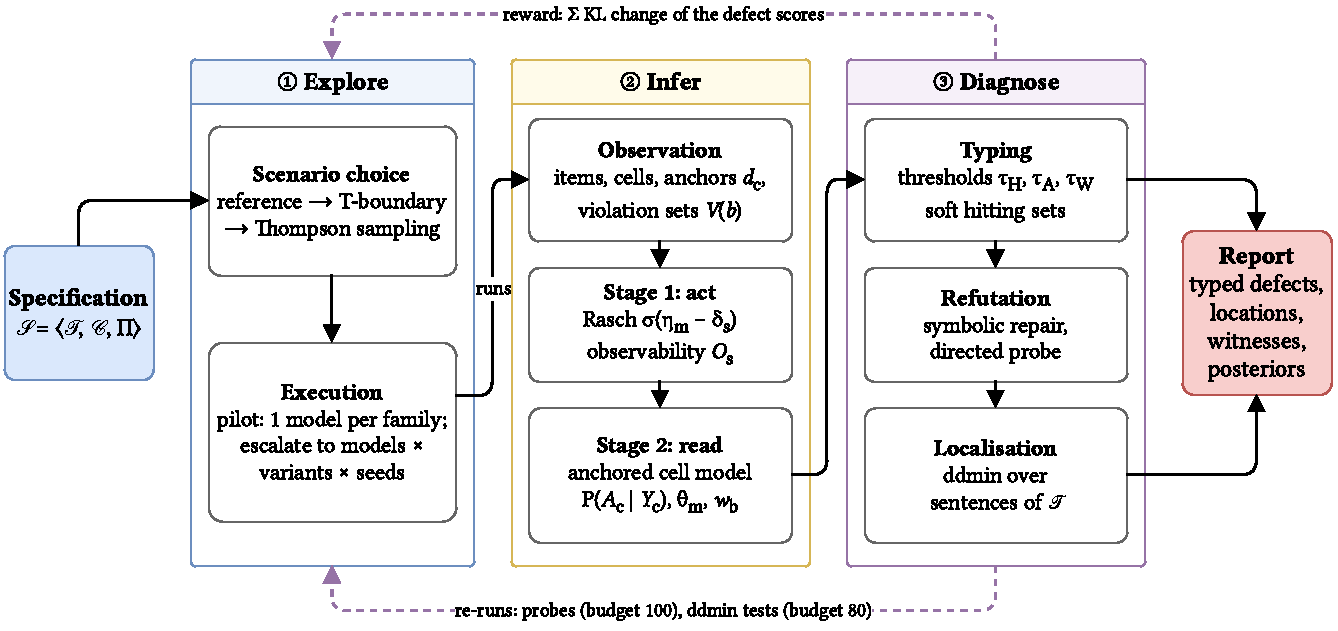
\includegraphics[width=\textwidth]{figures/drawio/pipeline.pdf}
\caption{Overview of \specdx. Each round explores a scenario, infers what the population's runs say about every cell, and diagnoses typed defects. Solid arrows show one round. Dashed arrows show the feedback: the change in the defect scores rewards the scenario choice, and refutation and localisation request further runs within their own budgets.}
\label{fig:pipeline}
\end{figure}

\subsection{Execution and observation}
\label{sec:approach-observe}

\paragraph{Neutral harness.} Each interpreter runs the process step by step with the tools of the step's digital employee. It works against a real PostgreSQL database with the specification's guardrails installed. It reads $\Tell$ through a retrieval tool: BM25 over 300-word chunks, $k=5$ per query.

Small open models sometimes write a tool call as text, or end a step without acting. A neutral harness handles both cases, and its texts contain no business value or rule:
\begin{itemize}[leftmargin=*]
\item \textbf{Tool calls written as text.} A call written as text is parsed and executed only if it names one of the step's tools and its arguments validate against that tool's schema.
\item \textbf{Steps that end without acting.} The harness may remind the model at most twice that it has not used a tool. The model remains free to answer that it is done.
\end{itemize}

\paragraph{What is recorded.} For each run, \specdx records the behaviour $b$, its violation set $V(b)$ from~\eqref{eq:violset}, and, for each item $s$, the act indicator
\begin{equation}
\label{eq:act}
a_{bs}=\one\bigl[\text{step } s \text{ ended } \textsf{done}\bigr]\cdot\one\bigl[\text{$b$ wrote at least one new row or event in the slice of } s\bigr].
\end{equation}
A step that errs, times out, is refused or writes nothing has $a_{bs}=0$.

For every cell $c$ that item $s$ may write, an acted behaviour also contributes a reading $y_{bc}$. Readings are normalised syntactically only, by Unicode NFC, trimming, whitespace folding, casefolding and canonical numerals. No semantic mapping is applied, so \textit{draft} and \textit{Nháp} remain different readings, and the model decides whether one of them is an interpreter error.

Rows are matched to golden rows by natural key. A key column whose golden values never occur in $\Tell$ is treated as generated by the executor, and its rows are matched on the remaining locked foreign keys instead.

\subsection{Stage 1: who acts, and where}
\label{sec:approach-act}

A model that never acts at an item says nothing about how it reads the item. Treating silence as disagreement was the main failure of our first prototype. \specdx therefore separates \emph{acting} from \emph{reading}. Stage 1 is a Rasch model~\cite{rodriguez2021evaluation,lalor2016building} of the act indicator:
\begin{equation}
\label{eq:rasch}
\Prob(a_{bs}=1)=\sigma\bigl(\eta_{m(b)}-\delta_s\bigr),
\end{equation}
where $\eta_m$ is model $m$'s capability to act and $\delta_s$ is the difficulty of item $s$. It is fitted by penalised maximum likelihood with an $L_2$ penalty $\lambda=1$ on $\eta$ and $\delta$, and with $\sum_s\delta_s=0$ fixed. The \emph{observability} of an item is the population's mean probability of acting,
\begin{equation}
\label{eq:observability}
O_s=\frac{1}{|\Models|}\sum_{m\in\Models}\sigma(\eta_m-\delta_s).
\end{equation}
An item is \emph{observable} when $O_s\ge\omega=0.3$ and at least $m_{\min}=3$ behaviours acted on it. Only acted behaviours contribute readings, and a finding whose clauses are not all relevant to observable items goes to an \emph{Unobservable} list. This list is reported, but it is never typed or scored. \Cref{prop:noaction} in \cref{sec:theory} shows that abstaining is the only calibrated answer in that case.

\subsection{Stage 2: the anchored cell model}
\label{sec:approach-model}

The anchored cell model is the core of \specdx. It answers \textbf{Q1}: given the readings of a cell by interpreters of differing competence, which readings does $\Tell$ admit?

\paragraph{Candidate values and latent sets.} For each cell $c$, the candidate set $V_c$ is built in three steps:
\begin{enumerate}[leftmargin=*]
\item it starts with the anchor $d_c$, if the cell is anchored;
\item it adds the most frequent observed readings, up to $K_{\max}=6$ values in all;
\item it adds one bucket \other for every remaining reading.
\end{enumerate}
The latent set $A_c$ ranges over
\begin{equation}
\label{eq:sets}
\Sets_c=\bigl\{\{x\}:x\in V_c^\circ\bigr\}\;\cup\;\bigl\{\{x,y\}:x\neq y\in V_c^\circ\bigr\}\;\cup\;\{\emptyset\},\qquad V_c^\circ=V_c\setminus\{\other\},
\end{equation}
which gives at most $6+15+1=22$ candidate sets per cell. \other never belongs to $A_c$.

\paragraph{Prior over sets.} We call the three ways a set can depart from the anchor its \emph{defect forms}:
\begin{itemize}[leftmargin=*]
\item \emph{mis}, a single value other than $d_c$;
\item \emph{amb}, a two-value set;
\item $\emptyset$, the empty set.
\end{itemize}
On an anchored cell, the prior keeps mass $1-\pi$ on the anchor and splits $\pi$ among the forms:
\begin{equation}
\label{eq:setprior}
\Prob(A_c=A)=
\begin{cases}
1-\pi, & A=\{d_c\},\\[2pt]
\pi\,s_f\,/\,N_f(c), & A \text{ of form } f\in\{\textit{mis},\textit{amb},\emptyset\},
\end{cases}
\end{equation}
where $s_{\textit{mis}}+s_{\textit{amb}}+s_\emptyset=1$ and $N_f(c)$ is the number of candidate sets of form $f$ at $c$. On an unanchored cell, the single values share $1-\pi$ uniformly, and $\pi$ is split between pairs and $\emptyset$ in the ratio $s_{\textit{amb}}:s_\emptyset$.

\paragraph{Reading model.} Let behaviour $b$ come from model $m=m(b)$. Its \emph{accuracy} at cell $c$ is
\begin{equation}
\label{eq:accuracy}
p_{m,c}=\sigma\bigl(\alpha_m-\beta_{g(c)}\bigr),
\end{equation}
where $\alpha_m$ is the model's ability and $\beta_g$ is the difficulty of the cell's group. The group $g(c)$ is the column of a value cell (pooled over rows and scenarios), the kind and reference of an event cell, and the clause of a constraint cell. Given $A_c$, the reading $y_{bc}$ is generated by
\begin{equation}
\label{eq:reading}
\Prob\bigl(y_{bc}=y\mid A_c=A\bigr)=
\begin{cases}
p_{m,c}\,\dfrac{\one[y\in A]}{|A|}+\bigl(1-p_{m,c}\bigr)\,\tilde\varepsilon_c^{A}(y), & A\neq\emptyset,\\[8pt]
\varepsilon_c(y), & A=\emptyset,
\end{cases}
\qquad
\tilde\varepsilon_c^{A}(y)=\frac{\varepsilon_c(y)\,\one[y\notin A]}{1-\varepsilon_c(A)} .
\end{equation}
In words: with probability $p_{m,c}$, the interpreter reads the cell faithfully and picks one of the admissible values uniformly. Otherwise it errs, and its error is drawn from a cell-specific error distribution $\varepsilon_c$ \emph{restricted to values outside $A$}. When $\Tell$ says nothing ($A=\emptyset$), no reading is faithful, and all models draw from the same $\varepsilon_c$.

Three design choices distinguish~\eqref{eq:reading} from the classical Dawid--Skene~\cite{dawid1979maximum} and GLAD~\cite{whitehill2009whose} models.
\begin{enumerate}[leftmargin=*,label=(\roman*)]
\item \textbf{Set-valued truth.} The truth is a set, which may hold two values or none. This is what lets the model express ambiguity and silence.
\item \textbf{Accuracy is a probability of landing in the truth.} Because the error distribution is truncated to $V_c\setminus A$, error mass can never sit on an admissible value, and $p_{m,c}$ is exactly $\Prob_m(y\in A)$. In an earlier version, the error distribution was allowed to cover the admissible values. The data then fitted a whole one-parameter family of (accuracy, error) pairs equally well, and accuracy collapsed to the share of the plurality class. The truncation removes that degeneracy.
\item \textbf{The specification is one more rater.} The anchor enters only through the prior~\eqref{eq:setprior}, so a cell whose anchor is consistently contradicted by competent readers can move its posterior away from $d_c$.
\end{enumerate}

\paragraph{Parameter priors.} The parameters receive weakly informative priors:
\begin{equation}
\label{eq:paramprior}
\alpha_m\sim\Norm(\mu_\alpha,\sigma_\alpha^2),\qquad
\beta_g\sim\Norm(0,\tau^2),\qquad
\varepsilon_c\sim\Dir\bigl(\kappa\,u_c\bigr),
\end{equation}
where $u_c$ is the flat distribution over $V_c$ and $\kappa=10$. The flat pool has a specific job. A free per-cell $\varepsilon_c$ lets the silence hypothesis $A_c=\emptyset$ fit any sharp split or mode, and in our simulation spikes it absorbed almost every true ambiguity. Pulling $\varepsilon_c$ towards a flat profile makes silence predict flat readings, so a sharp split identifies a pair and a sharp mode identifies a value (\cref{thm:t2prime}). The pool is a regularisation, not a claim that errors are flat: real errors concentrate, and \cref{sec:theory} and the simulation study examine what happens then.

\Cref{fig:graphical} summarises the generative model as a plate diagram.

\begin{figure}[t]
\centering
\resizebox{\textwidth}{!}{% Plate diagram of the anchored cell model.
\begin{tikzpicture}[
  every node/.style={font=\footnotesize},
  latent/.style={circle, draw, minimum size=8.5mm, inner sep=0pt},
  obs/.style={latent, fill=gray!25},
  param/.style={rectangle, inner sep=1pt},
  arr/.style={-{Latex[length=1.8mm]}, thick},
  plate/.style={draw, rounded corners=3pt, inner sep=6pt}]
\node[obs] (y) at (0,0) {$y_{bc}$};
\node[latent] (A) at (0,1.7) {$A_c$};
\node[obs] (d) at (-1.6,2.9) {$d_c$};
\node[param] (pi) at (1.6,2.9) {$\pi,\ s_f$};
\node[latent] (eps) at (2.0,0.9) {$\varepsilon_c$};
\node[param] (kap) at (3.6,0.9) {$\kappa,\ u_c$};
\node[latent] (al) at (-3.4,0) {$\alpha_m$};
\node[param] (mua) at (-5.2,0) {$\mu_\alpha,\sigma_\alpha$};
\node[latent] (be) at (-1.9,-1.75) {$\beta_g$};
\node[param] (tau) at (-3.7,-1.75) {$\tau$};
\node[latent, dashed] (p) at (-1.6,0.55) {$p_{m,c}$};
\draw[arr] (d) -- (A); \draw[arr] (pi) -- (A);
\draw[arr] (A) -- (y); \draw[arr] (eps) -- (y); \draw[arr] (kap) -- (eps);
\draw[arr] (mua) -- (al); \draw[arr] (tau) -- (be);
\draw[arr] (al) -- (p); \draw[arr] (be) -- (p); \draw[arr] (p) -- (y);
\node[plate, fit=(y), label={[font=\scriptsize]below right:acted $b$}] (pb) {};
\node[plate, fit=(pb)(A)(d)(eps)(p), label={[font=\scriptsize]above right:cells $c\in\Cells$}] {};
\node[plate, fit=(al), label={[font=\scriptsize]below:models $m\in\Models$}] {};
\node[plate, fit=(be), label={[font=\scriptsize]below:groups $g$}] {};
\node[align=left, font=\scriptsize, anchor=west] at (4.6,1.9) {%
  $A_c\in\Sets_c$: admissible readings\\
  $p_{m,c}=\sigma(\alpha_m-\beta_{g(c)})$ (deterministic)\\
  $y\mid A\neq\emptyset$: faithful w.p.\ $p_{m,c}$,\\
  \quad otherwise $\varepsilon_c$ restricted to $V_c\setminus A$\\
  $y\mid A=\emptyset$: drawn from $\varepsilon_c$};
\end{tikzpicture}
}
\caption{Plate diagram of the anchored cell model. Shaded nodes are observed: the readings $y_{bc}$ and the anchors $d_c$. The anchor enters only through the prior on the latent set $A_c$. Accuracy $p_{m,c}$ is a deterministic function of model ability and group difficulty.}
\label{fig:graphical}
\end{figure}

\paragraph{Posterior.} Let $\Theta=(\alpha,\beta,\varepsilon)$ and let $Y_c=\{y_{bc}\}$ be the readings of cell $c$ by acted behaviours. Under conditional independence of readings given $A_c$ and $\Theta$, the cell-level posterior is
\begin{equation}
\label{eq:post}
\Prob(A_c=A\mid Y_c,\Theta)=\frac{\Prob(A_c=A)\prod_{b}\Prob(y_{bc}\mid A,\Theta)}{\sum_{A'\in\Sets_c}\Prob(A_c=A')\prod_{b}\Prob(y_{bc}\mid A',\Theta)},
\end{equation}
and \specdx maximises the log posterior with every $A_c$ summed out,
\begin{equation}
\label{eq:map}
\mathcal{L}(\Theta)=\sum_{c\in\Cells}\log\sum_{A\in\Sets_c}\Prob(A_c=A)\prod_{b}\Prob(y_{bc}\mid A,\Theta)\;+\;\log p(\alpha)+\log p(\beta)+\log p(\varepsilon).
\end{equation}

\paragraph{Fitting by EM.} \specdx finds a MAP estimate of $\Theta$ by expectation--maximisation~\cite{dempster1977maximum}.

\emph{E-step.} For each cell, compute the posterior~\eqref{eq:post} over all candidate sets. Then compute, for each reading, the probability that it is faithful,
\begin{equation}
\label{eq:faithful}
r_{bc}=\sum_{A\neq\emptyset}\Prob(A_c=A\mid Y_c,\Theta)\cdot\frac{p_{m,c}\,\one[y_{bc}\in A]/|A|}{p_{m,c}\,\one[y_{bc}\in A]/|A|+(1-p_{m,c})\,\tilde\varepsilon_c^A(y_{bc})},
\end{equation}
and the probability that the cell is not silent, $q_c=1-\Prob(A_c=\emptyset\mid Y_c,\Theta)$.

\emph{M-step for ability and difficulty.} The expected complete-data log posterior in $(\alpha,\beta)$ is a penalised logistic regression. In it, each reading is a trial of accuracy with weight $q_c$ and fractional success $r_{bc}$:
\begin{equation}
\label{eq:mstep-ab}
(\alpha,\beta)\leftarrow\argmax_{\alpha,\beta}\sum_{c}\sum_{b}\Bigl[r_{bc}\,\eta_{m(b),c}-q_c\log\bigl(1+e^{\eta_{m(b),c}}\bigr)\Bigr]-\frac{\|\alpha-\mu_\alpha\|^2}{2\sigma_\alpha^2}-\frac{\|\beta\|^2}{2\tau^2},
\qquad \eta_{m,c}=\alpha_m-\beta_{g(c)} .
\end{equation}
\specdx solves~\eqref{eq:mstep-ab} by damped Newton steps, using the Schur complement of the diagonal $\beta$ block.

\emph{M-step for the error distributions.} An error reading under $A\neq\emptyset$ is a draw from $\varepsilon_c$ after any draws that fell inside $A$ have been rejected. The exact EM step therefore adds the expected rejected draws to the observed error counts. Let $N_c^{\textit{err}}(A)$ be the number of readings of $c$ outside $A$. The expected rejected draws on a value $k$ are
\begin{equation}
\label{eq:mstep-eps-rej}
R_c(k)=\sum_{A\ni k}\Prob(A_c=A\mid Y_c,\Theta)\,N_c^{\textit{err}}(A)\,\frac{\varepsilon_c(k)}{1-\varepsilon_c(A)} .
\end{equation}
The update is then
\begin{equation}
\label{eq:mstep-eps}
\varepsilon_c(k)\leftarrow\frac{E_c(k)+R_c(k)+\kappa\,u_c(k)}{\sum_{k'}\bigl[E_c(k')+R_c(k')\bigr]+\kappa},
\qquad E_c(k)=\sum_b(1-r_{bc})\,\one[y_{bc}=k] .
\end{equation}
This is the posterior mean under $\Dir(\kappa u_c)$, so the prior acts as exactly $\kappa$ pseudo-counts towards the flat pool.

\emph{Initialisation and stopping.} The likelihood~\eqref{eq:map} is multimodal. On our base data, more than half of the anchored cells are read off their anchor by every model, because nobody writes those rows. That is beyond the breakdown point of the median estimator in \cref{thm:t3}. EM therefore runs from five starts and keeps the fit with the highest $\mathcal{L}$:
\begin{itemize}[leftmargin=*]
\item the median start of \cref{thm:t3};
\item a common ability $\alpha_m\in\{0,1,2,3\}$ for every model.
\end{itemize}
Every start sets $\beta_g=0$ and $\varepsilon_c=u_c$. EM stops when the largest parameter change falls below $10^{-6}$, or after 200 iterations. Non-convergence is reported, never hidden.

\paragraph{Outputs.} The fit yields three kinds of output:
\begin{itemize}[leftmargin=*]
\item \textbf{Per cell:} the posterior over $A_c$, its MAP set and the posterior mass of each defect form.
\item \textbf{Per model:} the ability $\alpha_m$ and the accuracy $\theta_m=\sigma(\alpha_m)$ at a cell of median difficulty.
\item \textbf{Per behaviour:} a weight
\begin{equation}
\label{eq:weight}
w_b=\frac{1}{|\Cells_b|}\sum_{c\in\Cells_b}r_{bc},
\end{equation}
the mean probability that $b$'s readings are faithful, taken over the cells $\Cells_b$ it read.
\end{itemize}
No component of \specdx is switched on or off by a hard threshold on competence. Posterior quantities are used as weights throughout.

\subsection{Typing}
\label{sec:approach-typing}

This subsection answers \textbf{Q2}: how the posteriors become typed findings with witnesses. \Cref{fig:typing} summarises the decision flow; the paragraphs below give the details.

\begin{figure}[t]
\centering
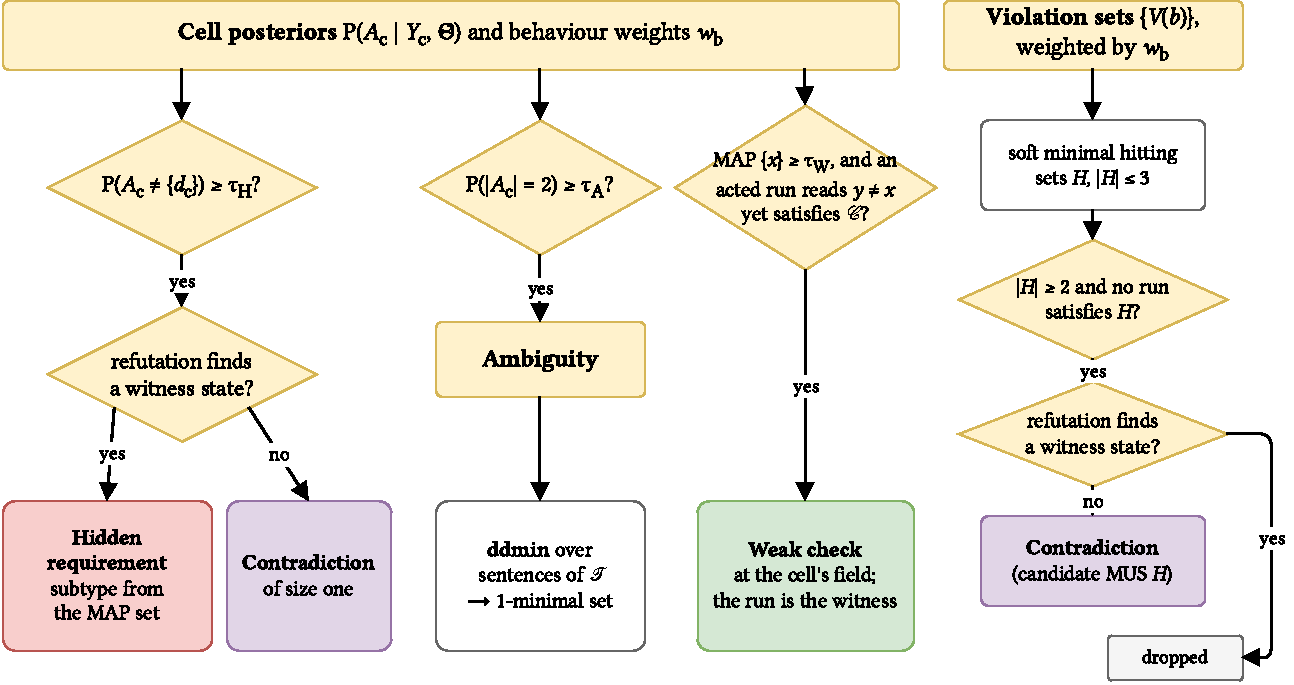
\includegraphics[width=\textwidth]{figures/drawio/typing.pdf}
\caption{Typing. The cell posteriors give hidden requirements, contradictions of size one, ambiguities and weak checks; the weighted violation sets give contradictions of two or more clauses. Every contradiction requires a failed refutation, and every ambiguity is localised in $\Tell$ by ddmin.}
\label{fig:typing}
\end{figure}

\paragraph{Hidden requirements and contradictions of size one.} An anchored cell is a candidate when its anchor is unlikely to be the whole truth:
\begin{equation}
\label{eq:hid-cand}
\Prob\bigl(A_c\neq\{d_c\}\mid Y_c,\hat\Theta\bigr)\ge\tau_H .
\end{equation}
The candidate then goes to \emph{refutation} (described below), which searches for a state that satisfies every applicable clause except the cell's own clause, together with a value of the cell other than $d_c$.
\begin{itemize}[leftmargin=*]
\item \textbf{A state is found.} The finding is a hidden requirement at the cell's clause, and its subtype follows the MAP form: mis-key for $\{a\}$, ambiguous-pick for a pair, unstated for $\emptyset$.
\item \textbf{No state is found.} The clause is a contradiction of size one.
\end{itemize}

\paragraph{Contradictions of two or more clauses.} If $b\models\Chk(\pi)\setminus V(b)$, then $V(b)$ is a \emph{correction set}: removing it makes the remaining clauses satisfiable. By the minimal hitting set duality of Reiter~\cite{reiter1987theory} and Liffiton and Sakallah~\cite{liffiton2008algorithms}, every minimal unsatisfiable subset is a minimal hitting set of the minimal correction sets. \specdx therefore treats every run as a free sample of a correction set, weighted by $w_b$. Let $\mathcal{V}_\pi=\{V(b)\}$ be the violation sets of the acted behaviours on $\pi$; each $V(b)$ is restricted to clauses relevant to items where $b$ acted. A set $H\subseteq\Chk(\pi)$ is a \emph{soft hitting set} when
\begin{equation}
\label{eq:sofths}
\frac{\sum_{b}w_b\,\one\bigl[H\cap V(b)\neq\emptyset\bigr]}{\sum_b w_b\,\one\bigl[V(b)\neq\emptyset\bigr]}\ge 1-\tau_{\textit{hs}},\qquad |H|\le 3 .
\end{equation}
\specdx enumerates minimal soft hitting sets with PySAT's \textsc{Hitman}~\cite{ignatiev2018pysat}, with $\tau_{\textit{hs}}=0.05$. It drops behaviours whose weight share is below $0.01$. A set $H$ with $|H|\ge 2$ becomes a contradiction candidate when every clause of $H$ is satisfied individually by some behaviour but no behaviour satisfies all of them together. The candidate is reported only if refutation fails. \Cref{fig:hitting} works through a small example.

\begin{figure}[t]
\centering
\resizebox{\textwidth}{!}{% Runs as sampled correction sets; a minimal hitting set is a candidate MUS.
\begin{tikzpicture}[
  every node/.style={font=\footnotesize},
  c/.style={minimum width=0.75cm, minimum height=0.48cm, draw=gray!50},
  hl/.style={c, fill=purple!15},
  arr/.style={-{Latex[length=2mm]}, thick},
  box/.style={draw, rounded corners=2pt, align=center, inner sep=4pt}]
\foreach \j/\n in {1/1,2/2,3/3,4/4} \node at (\j*0.75,0.5) {$\varphi_{\n}$};
\node at (4.15,0.5) {$w_b$};
\foreach \r/\row/\w in {1/{0,1,0,0}/0.9, 2/{0,0,1,0}/0.8, 3/{0,1,0,1}/0.7, 4/{1,0,1,0}/0.6, 5/{1,1,0,0}/0.9} {
  \node[anchor=east] at (0.3,-0.48*\r+0.48) {$V(b_{\r})$};
  \foreach \v [count=\j] in \row {
    \ifnum\j=2 \def\sty{hl}\else\ifnum\j=3 \def\sty{hl}\else\def\sty{c}\fi\fi
    \node[\sty] at (\j*0.75,-0.48*\r+0.48) {\ifnum\v=1 $\bullet$\fi};
  }
  \node at (4.15,-0.48*\r+0.48) {\w};
}
\node[font=\scriptsize, align=center, text width=4.2cm] at (2.0,-2.45) {each run $b$ satisfies $\Chk\setminus V(b)$, so $V(b)$ is a correction set};
\node[box, fill=purple!15] (H) at (7.0,-0.5) {minimal hitting set\\$H=\{\varphi_2,\varphi_3\}$\\covers all weight};
\node[box] (R) at (10.0,-0.5) {refutation: search\\for $w\models\{\varphi_2,\varphi_3\}$};
\node[box, fill=purple!25] (C) at (10.0,-2.0) {no witness:\\\Dcon $\{\varphi_2,\varphi_3\}$};
\node[box, fill=gray!10] (D) at (7.0,-2.0) {witness found:\\candidate dropped};
\draw[arr] (4.6,-0.5) -- (H);
\draw[arr] (H) -- (R);
\draw[arr] (R) -- (C);
\draw[arr] (R.south west) -- (D.north east);
\end{tikzpicture}
}
\caption{Runs as sampled correction sets. Every run violates $\varphi_2$ or $\varphi_3$, and each of the two is satisfied by some run, so $H=\{\varphi_2,\varphi_3\}$ is a minimal hitting set and a candidate MUS. It is reported as a contradiction only if refutation finds no state that satisfies both clauses.}
\label{fig:hitting}
\end{figure}

\paragraph{Refutation.} Refutation searches for a witness state $w$ with $w\models M$, along two routes.
\begin{itemize}[leftmargin=*]
\item \textbf{Symbolic repair.} Starting from the behaviours that violate the fewest clauses of $M$, a local search over the locked fields proposes edits. Each proposal is materialised in PostgreSQL inside a savepoint, so that derived values such as \texttt{fn\_reconcile} are computed by the real system. The search stops after at most 200 clause evaluations.
\item \textbf{Directed probe.} $\Tell$ is augmented with the goal of reaching a state that satisfies $M$, written from the clause descriptions. The three interpreters with the highest weight each make three attempts.
\end{itemize}
Refutation is sound: a returned witness proves that $M$ is satisfiable (\cref{prop:refute}). The reverse direction holds only probabilistically, so every contradiction is reported with the number of failed attempts.

\paragraph{Ambiguity.} A cell is reported as an ambiguity when
\begin{equation}
\label{eq:amb}
\Prob\bigl(|A_c|=2\mid Y_c,\hat\Theta\bigr)\ge\tau_A .
\end{equation}
Following \cref{def:defects}, an ambiguity whose pair excludes or includes the anchor is reported together with the corresponding hidden requirement.

\paragraph{Weak checks.} A cell $c$ is a weak-check candidate when two conditions hold:
\begin{enumerate}[leftmargin=*,label=(\roman*)]
\item its MAP set is a single value $\{x\}$ with posterior at least $\tau_W$;
\item some acted behaviour $b$ reads $y_{bc}\neq x$, yet satisfies every clause of $\Chk$ relevant to the item. This is checked symbolically on $b$'s state.
\end{enumerate}
Then $b$ witnesses~\eqref{eq:def-weak}: the population says $b$ is not admissible at $c$, and still no clause objects. The finding is located at the cell's column, or at the event's (kind, ref). Unanchored cells are the main source of weak checks. A weak check is suppressed on a cell that already reports a hidden requirement.

\paragraph{Differential reporting.} When a specification is compared with a reference version, as in the mutation study, only findings that are absent from the reference's report are kept. This applies the matching rules of \cref{sec:eval-design}.

\subsection{Localising ambiguity in the text}
\label{sec:approach-localise}

An ambiguity is only actionable if the author knows which sentences cause it. \specdx localises each reported ambiguity by delta debugging (ddmin)~\cite{zeller2002simplifying} over the sentences of $\Tell$ retrieved for the item's step. Let $T_s$ be those sentences. A test on a subset $U\subseteq T_s$ removes $U$ from $\Tell$ and re-runs one behaviour per (acting model, Tell variant) at seed 1. The oracle keeps the fitted $\hat\Theta$ fixed and asks whether the split persists:
\begin{equation}
\label{eq:ddmin-oracle}
\textsc{Test}(U)=\one\Bigl[\Prob\bigl(|A_c|=2\mid Y_c^{\Tell\setminus U},\hat\Theta\bigr)\ge\tau_A\Bigr].
\end{equation}
ddmin returns a 1-minimal set of sentences whose \emph{presence} is needed for the split. Its cost is $O(\log|T_s|)$ tests in favourable cases and $O(|T_s|^2)$ in the worst case. Localisation shares a budget of 80 runs per specification. An ambiguity whose test passes even with no candidate sentence, or whose localisation runs out of budget, is reported \emph{unlocalised}. It keeps its type with an empty location.

\subsection{Choosing scenarios}
\label{sec:approach-scenarios}

This subsection answers \textbf{Q3}. The scenarios come from a queue with three tiers, and each new scenario is run cheaply first. \Cref{fig:scenarios} illustrates the three mechanisms.

\begin{figure}[t]
\centering
\resizebox{\textwidth}{!}{% Scenario choice: T-boundary literals, Thompson sampling over scenario cells, and escalation.
\begin{tikzpicture}[
  every node/.style={font=\footnotesize},
  box/.style={draw, rounded corners=2pt, align=center, inner sep=3pt},
  arr/.style={-{Latex[length=2mm]}, thick}]
% (a) literal extraction
\node[box, fill=blue!8, text width=3.6cm] (s) at (0,1.6) {``\ldots\ \vi{chiết khấu} \underline{\vi{tối đa}} \textbf{5\%} \ldots''\\[-1pt]{\scriptsize (a sentence of $\Tell$)}};
\draw[thick] (-1.6,0.2) -- (1.6,0.2);
\foreach \x/\l in {-1.2/3,-0.6/4,0/5,0.6/6,1.2/7} {\draw (\x,0.12) -- (\x,0.28); \node[below, font=\scriptsize] at (\x,0.12) {\l};}
\foreach \x in {-0.6,0,0.6} \node[circle, fill=blue!60!black, inner sep=1.6pt] at (\x,0.2) {};
\node[font=\scriptsize] at (0,-0.45) {discount (\%): $\ell-1,\ \ell,\ \ell+1$};
\draw[arr] (s) -- (0,0.45);
\node[font=\footnotesize\bfseries] at (0,-1.45) {(a) T-boundary scenarios};
% (b) Thompson sampling over scenario cells
\begin{scope}[shift={(3.4,-0.3)}]
\foreach \i/\m/\s/\lab/\dr in {0/0.8/0.3/{below cap,\\1 receipt}/0.95, 1/1.1/0.4/{above cap,\\1 receipt}/1.25, 2/1.4/0.45/{at cap,\\2 receipts}/1.95} {
  \begin{scope}[shift={(\i*1.6,0)}]
  \draw[->, gray] (0,0) -- (0,2.2);
  \draw[thick, domain=0:2.1, samples=40, smooth, variable=\y, blue!60!black] plot ({0.9*exp(-((\y-\m)^2)/(2*\s*\s))},\y);
  \draw[red!70!black, thick] (-0.08,\dr) -- (0.5,\dr);
  \node[font=\scriptsize, align=center] at (0.35,-0.35) {\lab};
  \end{scope}}
\node[font=\scriptsize, rotate=90] at (-0.35,1.1) {reward \textit{IG}};
\draw[red!70!black, thick] (3.3,2.55) -- (3.6,2.55) node[right, font=\scriptsize, black] {draw};
\draw[blue!60!black, thick] (0.1,2.55) -- (0.4,2.55) node[right, font=\scriptsize, black] {posterior};
\draw[rounded corners=2pt, very thick, red!70!black] (3.0,-0.85) rectangle (4.3,2.3);
\end{scope}
\node[font=\footnotesize\bfseries] at (5.1,-1.45) {(b) Thompson sampling over scenario cells};
% (c) escalation
\begin{scope}[shift={(10.0,0)}]
\node[box, fill=gray!10] (pl) at (0,1.75) {pilot: 1 model per family,\\variant 0, seed 1};
\node[box, fill=yellow!20, text width=3.1cm] (tr) at (0,0.65) {new correction set, or\\$\ge2$ acted readings?};
\node[box, fill=green!15] (fu) at (0,-0.45) {full population:\\models $\times$ 3 variants $\times$ 3 seeds};
\draw[arr] (pl) -- (tr); \draw[arr] (tr) -- node[right, font=\scriptsize] {yes} (fu);
\draw[arr] (tr.east) -- ++(0.35,0) node[right, font=\scriptsize, align=left] {no:\\next\\scenario};
\node[font=\footnotesize\bfseries] at (0,-1.45) {(c) sequential escalation};
\end{scope}
\end{tikzpicture}
}
\caption{Choosing scenarios. (a)~A numeric literal next to a comparison keyword in $\Tell$ adds boundary values to a parameter's domain. (b)~Each scenario cell keeps a posterior over the information gain of running it; one draw per cell is taken and the largest wins (values illustrative). (c)~A new scenario first runs a pilot and is escalated to the full population only if the pilot is informative.}
\label{fig:scenarios}
\end{figure}

\paragraph{Reference and boundary scenarios.} The queue starts with the reference scenarios of $\Chk$. Next come \emph{T-boundary} scenarios. \specdx extracts every numeric literal in $\Tell$ that appears in the same sentence as a comparison keyword, such as ``\vi{tối đa}'' (at most) or ``\vi{vượt quá}'' (exceeds). It binds percentages to the discount parameter and quantities to the received quantity. Each bound literal $\ell$ adds $\ell-1$, $\ell$ and $\ell+1$ to the parameter's domain. At most 12 such scenarios are queued, each varying one parameter from the anchor scenario.

\paragraph{Thompson sampling over scenario cells.} After the queue, \specdx selects scenarios by Thompson sampling~\cite{thompson1933likelihood,russo2018tutorial}. Scenarios are grouped into \emph{scenario cells} $\zeta(\pi)$. A cell combines the structural parameters, such as the number of receipts per order, with boundary flags that say whether each parameter lies below, at or above its nearest literal. Each scenario cell keeps a Normal--Gamma posterior over the reward of running a scenario from it. The reward is the realised information gain, the total binary Kullback--Leibler divergence between the typed defect scores after and before the round:
\begin{equation}
\label{eq:reward}
\textit{IG}(\pi)=\sum_{h\in\mathcal{H}}\KL\bigl(\textit{Bern}(\rho_h^{\text{after}})\,\big\|\,\textit{Bern}(\rho_h^{\text{before}})\bigr),
\end{equation}
where $\mathcal{H}$ is the set of defect hypotheses, that is, the candidate cells and clause sets, and $\rho_h$ is the score of hypothesis $h$. Untried scenario cells are explored first. Afterwards, \specdx draws one mean per open cell from its posterior, takes the cell with the largest draw and runs an unvisited scenario from it. The search stops when every open cell has been tried and the largest posterior mean reward falls below $\epsilon=0.01$ nats, or when the budget runs out.

\paragraph{Sequential escalation.} Each new scenario first runs a \emph{pilot}: one model per family, Tell variant 0, seed 1. It is escalated to the full population (all models $\times$ 3 variants $\times$ 3 seeds) only if the pilot shows one of two things:
\begin{itemize}[leftmargin=*]
\item a correction set not seen before;
\item two or more distinct acted readings at some item.
\end{itemize}
Disagreement among non-acting views does not count, because a difference in capability is not a difference in reading.

\subsection{The main loop}

\Cref{alg:specdx} puts the components together. It is deterministic given the seeds and the run cache: runs are keyed by a content digest of the specification, the scenario, the interpreter and the model's weights digest, so a resumed or re-run study reuses every run.

\begin{algorithm}[t]
\caption{\specdx}
\label{alg:specdx}
\small
\begin{algorithmic}[1]
\Require specification $\Spec=\langle\Tell,\Chk,\Scen\rangle$, population $\Pop$, budgets $B_{\textit{pop}},B_{\textit{probe}},B_{\textit{loc}}$
\Ensure ranked typed defects with locations and witnesses
\State $\Chk'\gets\textsc{Lift}(\Chk,\Scen)$;\; $Q\gets\textsc{Reference}(\Scen)\cdot\textsc{TBoundary}(\Tell,\Scen)$
\State $\mathcal{R}\gets\emptyset$;\; $\textit{seen}\gets\emptyset$;\; $\rho\gets\emptyset$ \Comment{runs, correction sets, scores}
\While{$B_{\textit{pop}}>0$ \textbf{and not} \textsc{Exhausted}(bandit, $\epsilon$)}
  \State $\pi\gets Q.\textsc{pop}()$ \textbf{or} \textsc{ThompsonChoose}(bandit)
  \State $\mathcal{R}_\pi\gets\textsc{Run}(\textsc{Pilot}(\Pop),\pi)$
  \If{$\exists b\in\mathcal{R}_\pi: V(b)\notin\textit{seen}$ \textbf{or} pilot disagrees on an acted item}
    \State $\mathcal{R}_\pi\gets\mathcal{R}_\pi\cup\textsc{Run}(\Pop,\pi)$ \Comment{escalation}
  \EndIf
  \State $\mathcal{R}\gets\mathcal{R}\cup\mathcal{R}_\pi$;\; $\textit{seen}\gets\textit{seen}\cup\{V(b):b\in\mathcal{R}_\pi\}$
  \State $(\eta,\delta,O)\gets\textsc{FitRasch}(\mathcal{R})$ \Comment{\cref{eq:rasch,eq:observability}}
  \State $(\hat\Theta,\{\Prob(A_c\mid Y_c)\},w)\gets\textsc{FitAnchored}(\mathcal{R}, O)$ \Comment{\cref{eq:map,eq:faithful,eq:mstep-ab,eq:mstep-eps}}
  \State $D\gets\textsc{TypeCells}(\tau_H,\tau_A,\tau_W)\cup\textsc{SoftMHS}(\{V(b)\},w)$ \Comment{\cref{eq:hid-cand,eq:sofths,eq:amb}}
  \ForAll{candidates $M\in D$ needing refutation, by descending score}
    \State \textsc{Refute}$(M)$ within $B_{\textit{probe}}$ \Comment{repair, then directed probe}
  \EndFor
  \State $\rho'\gets\textsc{Scores}(D)$;\; \textsc{UpdateBandit}$(\zeta(\pi),\textit{IG}(\rho',\rho))$;\; $\rho\gets\rho'$ \Comment{\cref{eq:reward}}
\EndWhile
\ForAll{ambiguities in $D$, by descending score}
  \State \textsc{DDMin}$(T_s,\textsc{Test})$ within $B_{\textit{loc}}$ \Comment{\cref{eq:ddmin-oracle}}
\EndFor
\State \Return $\textsc{Rank}(D)$ with posteriors, witnesses, refutation attempts and the Unobservable list
\end{algorithmic}
\end{algorithm}

\paragraph{Cost.} With the default budgets of 200 population runs, 100 probe runs and 80 localisation runs, one specification costs at most 380 runs. Each EM fit takes $O(I\cdot\sum_c|\Sets_c|\cdot n_c)$ time, where $I\le200$ is the number of iterations and $n_c$ is the number of readings of cell $c$. In practice it is negligible next to the cost of running the interpreters.

\subsection{Hyper-parameters and pre-registration}
\label{sec:approach-hparams}

\Cref{tab:hparams} lists every hyper-parameter. They fall into two groups:
\begin{itemize}[leftmargin=*]
\item \textbf{Fixed by design.} These were set before any experiment.
\item \textbf{Chosen by simulation.} The defect prior, the ability prior, the difficulty spread and the three typing thresholds were chosen by a fixed selection rule on simulated specifications calibrated to base runs only (\cref{sec:eval-design}). They were then frozen in a pre-registration that a test pins.
\end{itemize}
No hyper-parameter of \specdx was chosen on a seeded or real defect.

\begin{table}[t]
\caption{Hyper-parameters of \specdx. Values marked $^\dagger$ were selected by the pre-registered simulation rule (\cref{sec:eval-sim}) and frozen before any mutant was run; all others were fixed by design.}
\label{tab:hparams}
\small
\begin{tabular}{@{}llr@{}}
\toprule
Component & Parameter & Value \\
\midrule
Population & temperature; Tell variants; seeds & $0.7$; $\{0,1,2\}$; $\{1,2,3\}$ \\
           & models per family / in total / families & $\le2$ / $\le4$ / $\ge2$ \\
Stage 1    & $L_2$ penalty $\lambda$; observability $\omega$; $m_{\min}$ & $1.0$; $0.3$; $3$ \\
Cells      & $K_{\max}$; $|A_c|_{\max}$ & $6$; $2$ \\
Anchored model & error concentration $\kappa$ (flat pool) & $10$ \\
           & defect prior $\pi$; shares $(s_{\textit{mis}},s_{\textit{amb}},s_\emptyset)$ & $0.2^\dagger$; $(0.4,0.3,0.3)^\dagger$ \\
           & ability prior $(\mu_\alpha,\sigma_\alpha)$; difficulty s.d.\ $\tau$ & $(1.0,1.0)^\dagger$; $1.0^\dagger$ \\
           & EM tolerance; maximum iterations; starts & $10^{-6}$; $200$; $5$ \\
Typing     & $\tau_H$; $\tau_A$; $\tau_W$ & $0.5^\dagger$; $0.3^\dagger$; $0.9^\dagger$ \\
           & soft hitting tolerance $\tau_{\textit{hs}}$; max size; min weight share & $0.05$; $3$; $0.01$ \\
Refutation & repair evaluations; probe interpreters $\times$ attempts & $200$; $3\times3$ \\
Scenarios  & T-boundary scenarios; stopping $\epsilon$ & $\le12$; $0.01$ nats \\
Budgets    & population / probe / localisation runs & $200$ / $100$ / $80$ \\
\bottomrule
\end{tabular}
\end{table}

\section{Theory}
\label{sec:theory}

This section asks when the anchored cell model can recover the latent set $A_c$ from readings, and how many readings it needs. All statements are per cell, so we drop the index $c$. Proofs are in \cref{app:proofs}.

\subsection{Assumptions}

\begin{description}[leftmargin=2.2em,style=nextline]
\item[(A1) Independence.] Given $A$ and $\Theta$, the readings of one model are independent. They need not be identically distributed across Tell variants. $P_m$ then denotes the variant-averaged reading distribution of model $m$.
\item[(A2) Accuracy parametrisation.] If $A\neq\emptyset$, then $P_m(A)=p_m$, faithful readings are uniform on $A$, and $|A|\le2$.
\item[(A3) Shared errors.] The error distribution $\varepsilon$, restricted to $V\setminus A$, is the same for every model at the cell.
\item[(A4) Monotone accuracy.] $p_{m,c}=\sigma(\alpha_m-\beta_{g(c)})$. The order of models by accuracy is therefore the same at every cell.
\item[(A5) Silence.] If $A=\emptyset$, every model reads from $\varepsilon$: competence does not help where $\Tell$ says nothing.
\end{description}

(A2) and (A4) are modelling choices. (A1) holds approximately because readings come from separate runs with distinct seeds and variants. (A3) and (A5) are the substantive assumptions, and both may fail. Errors of different LLMs are known to be correlated~\cite{kim2025correlated,goel2025great}, which favours (A3) at the population level, but the \emph{shape} of errors is not flat. A strong model may also guess a value that $\Tell$ does not state, from domain knowledge. We return to both failures in \cref{sec:theory-scope} and test them in simulation.

\subsection{Accuracy-gradient signatures}

The key observation is that each defect form changes the reading distribution in a different way as accuracy grows. Take two models with $p_1>p_2$, write $\Delta=p_1-p_2$, and let
\begin{equation}
\label{eq:contrast}
D(y)=P_1(y)-P_2(y).
\end{equation}

\begin{lemma}[Signatures]
\label{lem:signatures}
Under (A2), (A3) and (A5), let $\tilde\varepsilon=\varepsilon(\cdot\mid V\setminus A)$. Then
\begin{equation}
\label{eq:signature}
D(y)=
\begin{cases}
\Delta\Bigl(\dfrac{\one[y\in A]}{|A|}-\tilde\varepsilon(y)\Bigr), & A\neq\emptyset,\\[8pt]
0, & A=\emptyset .
\end{cases}
\end{equation}
\end{lemma}

The lemma gives a simple rule:
\begin{itemize}[leftmargin=*]
\item the mass on an admissible value rises with accuracy;
\item the mass on an error value falls;
\item when $\Tell$ is silent, nothing depends on accuracy at all.
\end{itemize}
\Cref{tab:signatures} lists the signs, and \cref{fig:signatures} draws the curves.

The sign difference matters most for ambiguity. A concentrated error $a\notin A$ and the second reading $a\in A$ of an ambiguous cell can have the same frequency at one accuracy level. They move in opposite directions as accuracy grows, which is what separates them.

\begin{table}[t]
\caption{Accuracy-gradient signatures (\cref{lem:signatures}) for two models with $p_1>p_2$ and $\Delta=p_1-p_2$.}
\label{tab:signatures}
\small
\begin{tabular}{@{}lll@{}}
\toprule
Form of $A$ & $D(y)$ for $y\in A$ & $D(y)$ for $y\notin A$ \\
\midrule
$\{x\}$ (no defect if $x=d$; mis-key otherwise) & $\Delta>0$ & $-\Delta\,\tilde\varepsilon(y)\le0$ \\
$\{x,a\}$ (ambiguity) & $\Delta/2>0$ & $-\Delta\,\tilde\varepsilon(y)\le0$ \\
$\emptyset$ (silence) & --- & $0$ for every $y$ \\
\bottomrule
\end{tabular}
\end{table}

\begin{figure}[t]
\centering
\begin{tikzpicture}
\begin{groupplot}[
  group style={group size=4 by 1, horizontal sep=9mm, y descriptions at=edge left},
  width=0.29\textwidth, height=0.25\textwidth,
  xmin=0.3, xmax=1, ymin=0, ymax=1,
  xlabel={accuracy $p$}, ylabel={$P_m(y)$},
  xtick={0.4,0.6,0.8,1}, ytick={0,0.25,0.5,0.75,1},
  tick label style={font=\scriptsize}, label style={font=\scriptsize}, title style={font=\footnotesize},
  every axis plot/.append style={thick, samples=2, domain=0.3:1}]
\nextgroupplot[title={$A=\{x\}$, flat errors}]
  \addplot[black] {x};
  \addplot[black, dashed] {(1-x)/3};
\nextgroupplot[title={$A=\{x,a\}$, flat errors}]
  \addplot[black] {x/2};
  \addplot[blue, densely dotted, very thick] {x/2};
  \addplot[black, dashed] {(1-x)/2};
\nextgroupplot[title={$A=\{x\}$, concentrated error}]
  \addplot[black] {x};
  \addplot[red, densely dashdotted, very thick] {0.84*(1-x)};
  \addplot[black, dashed] {0.08*(1-x)};
\nextgroupplot[title={$A=\emptyset$}]
  \addplot[black, dashed] {0.25};
\end{groupplot}
\end{tikzpicture}
\caption{Accuracy-gradient signatures drawn from \cref{eq:reading} with $|V|=4$. Solid lines show admissible values and dashed lines show error values. In the second panel, the dotted blue line is the second admissible value of an ambiguous cell. In the third panel, the dash-dotted red line is an error value holding $84\%$ of the error mass. At $p\approx0.63$, the blue line in the second panel and the red line in the third have similar heights, but they have opposite slopes. Under silence, no reading depends on accuracy. The curves are analytical, not experimental.}
\label{fig:signatures}
\end{figure}

\subsection{Identifiability}

\begin{theorem}[T1: single value, one model]
\label{thm:t1}
Let $A=\{x\}$, and suppose the plurality condition
\begin{equation}
\label{eq:pc}
p_m>(1-p_m)\max_{y}\tilde\varepsilon(y)\tag{PC$_m$}
\end{equation}
holds. Then $x$ is the unique mode of $P_m$, and $p_m=P_m(x)$.
\end{theorem}

\begin{theorem}[T2: all forms from two models]
\label{thm:t2}
Under (A1)--(A5), with $p_1>p_2$,
\begin{equation}
\label{eq:t2}
A=\{y\in V:D(y)>0\}.
\end{equation}
In particular, $A=\emptyset$ exactly when $D\equiv0$. Under (A4), $\Delta_c>0$ at every cell whenever $\alpha_1\neq\alpha_2$. Hence the forms no defect, mis-key, ambiguity and silence are identified at every cell from any two models of distinct ability.
\end{theorem}

\Cref{thm:t2} needs an accuracy contrast. The flat error pool of \cref{eq:paramprior} gives a second route that needs only one model.

\begin{theorem}[T2$'$: all forms from one model with a known error pool]
\label{thm:t2prime}
Let $\varepsilon=u$ be flat over $V$, with $K=|V|$, and let $p$ be the model's accuracy at the cell.
\begin{itemize}[leftmargin=*]
\item If $A\neq\emptyset$, then $P_m(y)=p/|A|$ for $y\in A$, and $P_m(y)=(1-p)/(K-|A|)$ for $y\notin A$.
\item If $A=\emptyset$, then $P_m$ is flat at $1/K$.
\end{itemize}
Hence $A$ is identified from $P_m$ alone whenever
\begin{equation}
\label{eq:t2prime}
p\neq|A|/K,
\end{equation}
that is, whenever the faithful share differs from what chance would give.
\end{theorem}

\Cref{thm:t1,thm:t2,thm:t2prime} assume that accuracies are known or can be contrasted. The anchors make this possible without labels, as long as most anchors are correct.

\begin{theorem}[T3: model contrasts from anchors]
\label{thm:t3}
At an anchored cell with $A_c=\{d_c\}$, the logit contrast
\begin{equation}
\label{eq:t3}
\ell_c\defeq\logit P_{1,c}(d_c)-\logit P_{2,c}(d_c)=\alpha_1-\alpha_2
\end{equation}
is the same at every non-defective anchored cell. If more than half of the anchored cells are non-defective, then $\median_c\ell_c=\alpha_1-\alpha_2$. The model order and the contrasts are therefore identified, even where \eqref{eq:pc} fails at individual cells: the estimator has a breakdown point of $\tfrac12$. The levels $\alpha_m$ are identified under the location constraint that $\median\beta_{g(c)}=0$ over the non-defective anchored cells.
\end{theorem}

\Cref{thm:t3} is also the reason for one of the EM starts (\cref{sec:approach-model}). When defects are not sparse, it is no longer guaranteed, and the multi-start procedure guards against the resulting poor fixed points.

\subsection{Finite samples}

Population-level identifiability says nothing about how many runs are needed. The next theorem bounds the error of three simple decision rules. Let $n$ be the smaller number of readings per model at the cell, and $\hat P_m$ the empirical reading distributions.

\begin{theorem}[T4: finite-sample bounds]
\label{thm:t4}
Under (A1)--(A5):
\begin{enumerate}[leftmargin=*,label=(\alph*)]
\item \textbf{Two-model contrast.} The rule $\hat A=\{y:\hat D(y)>\Delta/4\}$ errs with probability at most
  \begin{equation}\label{eq:t4a}
  4|V|\exp\bigl(-n\Delta^2/32\bigr).
  \end{equation}
\item \textbf{Plug-in mode.} Under \eqref{eq:pc} with margin $\gamma=p-(1-p)\max_y\tilde\varepsilon(y)$, the mode of $\hat P_m$ differs from $x$ with probability at most
  \begin{equation}\label{eq:t4b}
  2|V|\exp\bigl(-n\gamma^2/2\bigr).
  \end{equation}
\item \textbf{Minimum distance.} Under \cref{thm:t2prime}, let $\gamma_{\min}$ be the smallest sup-norm distance between the predicted reading distributions of two candidate sets. The rule that picks the candidate closest to $\hat P_m$ errs with probability at most
  \begin{equation}\label{eq:t4c}
  2|V|\exp\bigl(-n\gamma_{\min}^2/2\bigr).
  \end{equation}
\end{enumerate}
\end{theorem}

The bounds are conservative: they come from Hoeffding's inequality~\cite{hoeffding1963probability} and a union bound. \specdx does not use these rules directly; it uses the MAP estimator with priors. The simulation study measures its actual power. The bounds still show which quantities matter.
\begin{itemize}[leftmargin=*]
\item \textbf{The accuracy gap and the number of readings.} The error rate falls exponentially in $n\Delta^2$. Pooling lifted cells across scenarios increases $n$.
\item \textbf{Concentrated errors.} An error that holds most of the error mass reduces $\gamma$ and hence the power of the single-model rules. This is why ambiguity, whose signature is weakest, benefits most from several models.
\item \textbf{The size of the candidate set.} The set size $|V|$ enters only logarithmically, so $K_{\max}=6$ costs little.
\end{itemize}

\subsection{Soundness of the logical components}

\begin{proposition}[Sound refutation]
\label{prop:refute}
If refutation returns a state $w$ on which every clause of $M$ evaluates to $\sat$, then $M$ is satisfiable, and $M$ is not a contradiction.
\end{proposition}

\begin{proposition}[No identification without action]
\label{prop:noaction}
Suppose that no acted behaviour touches the rows read by clause $\varphi$. Then every behaviour-based observation has the same distribution when $\varphi$ is a hidden requirement as when $\varphi$ is correct but unreachable by the population. No method that observes only behaviours can distinguish the two cases, and abstaining is the only calibrated output.
\end{proposition}

\Cref{prop:noaction} applies to every behaviour-based baseline in our study as much as to \specdx. It motivates both the Unobservable list of stage 1 and the observability-aware scoring of the evaluation (\cref{sec:eval-design}).

\subsection{Scope of the theory}
\label{sec:theory-scope}

\paragraph{Where the assumptions fail.}
\begin{itemize}[leftmargin=*]
\item \textbf{(A3): errors concentrate or differ by model.} The flat pool is then misspecified, and a concentrated error can look like the second reading of an ambiguous cell. \Cref{lem:signatures} shows that the two still differ in slope. With few models and small accuracy gaps, however, this difference is hard to see. The simulation study includes an arm that violates (A3).
\item \textbf{(A5): a strong model guesses an unstated value.} This only moves a finding from the \emph{unstated} to the \emph{mis-key} subtype. Both subtypes are hidden requirements, so the reported type does not change. The simulation includes an arm that violates (A5).
\end{itemize}

\paragraph{What the theory does not cover.} Contradictions are symbolic and are not covered by \cref{thm:t1,thm:t2,thm:t2prime,thm:t3,thm:t4}; \cref{prop:refute} covers them. Weak checks rest on \cref{thm:t1}: they need only a plurality margin at the cell, not an accuracy contrast.

\paragraph{The advantage depends on the regime.} Simple heuristics can match the anchored cell model in some regimes. Majority vote over models does well when accuracy is moderate and the population is small. Flagging every deviation from the anchor does well on hidden requirements, but it is blind to ambiguity. The evaluation therefore reports a full regime map instead of a single operating point (\cref{sec:results-rq1}).

\section{Evaluation Design}
\label{sec:eval-design}

\subsection{Research questions}

\begin{description}[leftmargin=2.6em,style=nextline]
\item[\rqref{1} Identifiability in practice.] Does the anchored cell model recover interpreter accuracy and the defect form of each cell under realistic noise, and in which regimes does it beat simpler aggregators?
\item[\rqref{2} Effectiveness on seeded defects.] How accurately does \specdx detect, type and localise seeded defects, compared with seven published baselines?
\item[\rqref{3} Real defects.] Does \specdx rediscover the defects recorded in the subject's history?
\item[\rqref{4} Cost-effectiveness.] How does effectiveness grow with the number of runs, and how does \specdx compare with the baselines at equal cost?
\item[\rqref{5} Ablation.] What does each component contribute?
\end{description}

\rqref{1} is answered by simulation, which needs no GPU and has a known ground truth. \rqref{2}--\rqref{5} are answered on the subject specification.

\subsection{Subject}
\label{sec:eval-subject}

\Cref{tab:subject} summarises the subject, the procure-to-pay specification of TonomyX CASE-0031 (\cref{sec:motivating}). We vendored TonomyX byte for byte at a fixed commit and never edit it. \specdx has its own PostgreSQL instance. The subject is demanding for three reasons:
\begin{itemize}[leftmargin=*]
\item $\Tell$ is long, written in Vietnamese and spread over several documents;
\item $\Chk$ mixes declarative invariants, procedural SQL and a golden state;
\item the process involves human approval gates. At each gate, the scenario fixes the decision, and a persona interpreter records it and carries out its consequences.
\end{itemize}

\begin{table}[t]
\caption{The subject specification.}
\label{tab:subject}
\small
\begin{tabular}{@{}lp{10.6cm}@{}}
\toprule
Part & Content \\
\midrule
$\Tell$ & Business-analysis document (97 pp.), demo description (46 pp.), software architecture document (18 pp.), three knowledge-base articles, business principles, tool catalogue, schema, scope table and tool refusal messages; served through a BM25 retrieval tool \\
$\Chk$ & 42 invariants, scenario expectations, golden end state over 26 tables, guardrail triggers and SQL policy functions, blank-column list, event vocabulary, scope table; executed on PostgreSQL 16 through nine gated tools \\
$\Scen$ & Ordered quantity, received quantity, requested discount, receipts per order; three reference scenarios (\textit{happy}, \textit{discount8}, \textit{grn12}); T-boundary and synthesised scenarios \\
Process & Interpreter steps by digital employees and human-gate personas, from sales order to payment \\
\bottomrule
\end{tabular}
\end{table}

A second subject, the airline and retail domains of $\tau^2$-bench~\cite{barres2026bench} with the repairs of its verified release as real defects, is designed but not yet built. We return to it in \cref{sec:discussion}.

\subsection{Interpreter population}

The population is chosen by an automatic, outcome-free capability screen. Each candidate model runs the base specification on the \textit{happy} scenario under three Tell variants and three seeds. The screen measures two things:
\begin{itemize}[leftmargin=*]
\item the \emph{act rate}, the fraction of interpreter steps with $a_{bs}=1$;
\item the \emph{valid-call rate}, the fraction of tool calls that validate against the tool's schema.
\end{itemize}
The screen never compares a run with $\Chk$, because doing so would be circular when $\Chk$ is the object under diagnosis. A model is admitted when its act rate is at least $0.3$ and its valid-call rate is at least $0.8$. The ranking keeps at most two models per family and four in total, from at least two families. If fewer than four models are admitted, the study stops.

\Cref{tab:population} lists the admitted population. All models run locally through Ollama 0.30.4 with pinned weight digests.

\begin{table}[t]
\caption{Interpreter population chosen by the capability screen. Screen statistics are filled in from the frozen screen results.}
\label{tab:population}
\small
\begin{tabular}{@{}llrrr@{}}
\toprule
Family & Model & Parameters & Act rate & Valid-call rate \\
\midrule
Qwen & \texttt{qwen3:30b-a3b} & 30B (3.3B active) & \tbd & \tbd \\
Qwen & \texttt{qwen2.5:14b} & 14B & \tbd & \tbd \\
OpenAI (open weights) & \texttt{gpt-oss:20b} & 21B (3.6B active) & \tbd & \tbd \\
Mistral & \texttt{mistral-small3.2:24b} & 24B & \tbd & \tbd \\
\bottomrule
\end{tabular}
\end{table}

\subsection{Seeded defects}
\label{sec:eval-mutants}

We seed defects with nine specification mutation operators, listed in \cref{tab:operators}. In the spirit of specification mutation~\cite{black2000mutation,jia2011analysis}, every operator edits only artefacts that the running system reads, so every mutant takes effect. Every state-level operator also emits a \emph{kill witness}: a state that proves the defect is real and can be activated. This removes the equivalent-mutant problem~\cite{schuler2011assessing}.

Each operator declares the rows, fields or steps its truth needs to be observed (\textit{observed at}). This is benchmark metadata and is never an input to any method.

\begin{table}[t]
\caption{Specification mutation operators, application sites and the development/test split (five development mutants per type, stratified, fixed seed).}
\label{tab:operators}
\small
\begin{tabular}{@{}llp{7.4cm}rr@{}}
\toprule
Type & Op. & Edit & Sites & Truth location \\
\midrule
\multirow{2}{*}{\Dcon} & C1 & Add an invariant that conflicts with an existing row-level equality invariant (same row and column, different value) & 6 & clause pair \\
 & C2 & Add a guardrail trigger that forbids a status the golden state requires & 3 & clause set \\
\multirow{2}{*}{\Dhid} & H1 & Change a locked value in the golden state, with no support in $\Tell$ & 5 & golden clause \\
 & H2 & Add an invariant demanding an event that $\Tell$ never motivates & 2 & clause \\
\multirow{3}{*}{\Damb} & A1 & Delete a disambiguating sentence of $\Tell$ & 3 & chunk \\
 & A2 & Replace a precise value in a sentence of $\Tell$ by a vague phrase & 3 & sentence \\
 & A3 & Add a knowledge-base article with an overlapping validity period and a different cap & 1 & sentences \\
\multirow{2}{*}{\Dweak} & W1 & Remove a column from the blank list and delete the invariant that guards it & 7 & field \\
 & W2 & Delete a golden event that the interpreter is told to log & 6 & event \\
\midrule
\multicolumn{3}{@{}l}{Total: 36 mutants; development split 20 (5 per type); test split 16 (4\,/\,2\,/\,2\,/\,8)} & 36 & \\
\bottomrule
\end{tabular}
\end{table}

\paragraph{Scorability.} A mutant can be detected by \emph{any} behaviour-based method only if the population reaches the place it changes (\cref{prop:noaction}). A mutant is therefore \emph{scorable} when, in the base specification's runs, at least $k=3$ acted behaviours touch its \textit{observed-at} targets. The scorable set is computed once from base runs, before any mutant runs, and it is the same for every method. The primary tables score scorable mutants. Secondary tables score all mutants and report how many were excluded per type.

\subsection{Real defects}

\Cref{tab:real} lists the real defects. R-SO and R-12 were described in \cref{sec:motivating}.
\begin{itemize}[leftmargin=*]
\item \textbf{R-DE.} The list of digital employees declares 15 of them, while the scope table grants capabilities to only nine. The mismatch is a hidden requirement wherever $\Tell$ assigns work to an employee without scope.
\item \textbf{R-DOC.} A documentation-only inconsistency that no behaviour can expose. It is used only for a qualitative check of the static reviewer.
\end{itemize}

\begin{table}[t]
\caption{Real defects from the subject's history.}
\label{tab:real}
\small
\begin{tabular}{@{}lp{6.6cm}p{3.4cm}l@{}}
\toprule
Id & Defect & Expected type & Scored \\
\midrule
R-SO & \texttt{SO-0031} stays \emph{\vi{Chờ duyệt}} after \texttt{APR-0102} is approved, while \texttt{PO-0015} moves to \emph{\vi{Đã duyệt}} & \Dhid (mis-key) & yes \\
R-12 & The schema allows several receipts per order; \texttt{fn\_reconcile} raises a cardinality error on that input & \Dcon & yes \\
R-DE & 15 digital employees declared; 9 granted scope & \Dhid where $\Tell$ assigns such work & yes \\
R-DOC & README states 33 invariants, the invariant file has 42; load orders differ & documentation only & no \\
\bottomrule
\end{tabular}
\end{table}

\subsection{Baselines}
\label{sec:eval-baselines}

We compare \specdx with the closest published method for each defect type, or for each component of \specdx. \Cref{tab:baselines} lists them. Three candidates were excluded because their code carries no licence: ClarifyGPT~\cite{mu2024clarifygpt}, SpecFix~\cite{jia2025automated} and AgentSuite/COBA~\cite{suh2026agentsuite}. We discuss them in \cref{sec:related}.

\begin{table}[t]
\caption{Baselines. ``Runs'' means the baseline consumes exactly \specdx's cached runs of the same specification, including synthesised scenarios; any bias this introduces favours the baseline.}
\label{tab:baselines}
\small
\begin{tabular}{@{}lp{4.1cm}p{4.6cm}l@{}}
\toprule
Id & Method & Input and adaptation & Types \\
\midrule
B1 & BenchGuard~\cite{tu2026who} & Definition audit of instruction, tests and solution, packaged per specification; original package; open models & all four \\
B2 & Who\&When~\cite{zhang2025which} & Failing runs as multi-agent logs; three original strategies plus a ``specification defect'' verdict; open models & \Dhid \\
B3 & IRT audit, forced ceiling~\cite{land2026auditing} & Models $\times$ cells/clauses from runs; likelihood-ratio indicator & \Dhid \\
B4 & Semantic entropy~\cite{farquhar2024detecting,kuhn2023semantic} & Discrete entropy of cell readings (pooled and per family); same ddmin localiser as \specdx & \Damb \\
B5 & MUS on $\Chk$ alone~\cite{ignatiev2018pysat,liffiton2008algorithms} & Symbolic repair from the golden state, no interpreters; minimal hitting sets & \Dcon \\
TI & GLAD~\cite{whitehill2009whose}, Dawid--Skene~\cite{dawid1979maximum} & Task $=$ cell, worker $=$ model; flag when the aggregate $\neq d_c$ & \Dhid \\
JEST & $N{+}1$-version rule~\cite{park2021jest} & Flag a cell/clause when the share of deviating models $\ge\tau$ & \Dhid \\
\midrule
B2-naive & Best single interpreter & Every violated clause flagged (secondary arm) & \Dhid \\
B3-2PL & 2PL IRT~\cite{rodriguez2021evaluation} & Negative discrimination flagged (secondary arm) & \Dhid \\
\bottomrule
\end{tabular}
\end{table}

\subsection{Metrics}

\paragraph{Matching.} A typed detection requires both a type match and a location match:
\begin{itemize}[leftmargin=*]
\item \textbf{Hidden requirement:} the reported clause equals the true clause.
\item \textbf{Contradiction:} the Jaccard index between the reported clause set and the true conflict set is at least $0.5$.
\item \textbf{Ambiguity:} the reported sentence set intersects the mutated sentences. For a deletion, any reported sentence in the chunk that held the deleted sentence matches.
\item \textbf{Weak check:} the reported fields include the field whose guard was removed.
\end{itemize}
Untyped matching drops the type requirement. Findings that are also present in the base specification's report are removed before matching (the differential).

\paragraph{Measures.} For each type, we report typed precision, recall and $F_1=2\,\textit{tp}/(2\,\textit{tp}+\textit{fp}+\textit{fn})$, computed in exact arithmetic so that ties are exact. We also report two threshold-free measures: average precision (AP) and Detection@$k$ for $k\in\{1,3,5\}$. Cost is counted in model requests, the one unit common to every method. Tokens and GPU time are added where they were recorded. Runs cached before the request counter existed are charged an upper bound, which overstates \specdx's cost.

\subsection{Fairness protocol}
\label{sec:eval-fairness}

\begin{itemize}[leftmargin=*]
\item \textbf{Same inputs.} Every method runs on the same base specification and mutants, and the run-consuming baselines read exactly \specdx's runs.
\item \textbf{Same models.} B1 and B2 run on each of the four population models with their original generation settings, and every call goes through one cached gateway.
\item \textbf{Selection on development data only.} For each baseline, the model, the strategy and the reporting threshold are chosen on the base and the 20 development mutants. The rule maximises mean typed $F_1$ over the types the baseline reports, with ties going to the smaller model and then the higher threshold. The choices are then frozen and committed.
\item \textbf{Conservative asymmetry.} \specdx's own thresholds come from simulation only (\cref{sec:eval-sim}), while the baselines are tuned on real development data.
\item \textbf{Two cost views.} Table A compares every method at its native protocol. Table B compares each LLM-based baseline with \specdx at the anytime checkpoint (25, 50, 100, 150 or 200 population runs) whose cost is closest to, and not above, the baseline's. Recording checkpoints never changes the final report, and a test verifies byte-identity.
\item \textbf{One-shot test split.} The test split is run once, only after the development gate is passed and the baseline pre-registration is committed with a clean working tree. The pre-registration records the hash of the gate configuration and its result, and the study refuses to run on a mismatch.
\end{itemize}

\subsection{Pre-registered protocol}
\label{sec:eval-sim}

The study proceeds through four go/no-go steps. Each step's pass criterion was written down before the step ran. \Cref{fig:protocol} shows the order of the steps and the comparison study that follows them.

\begin{figure}[t]
\centering
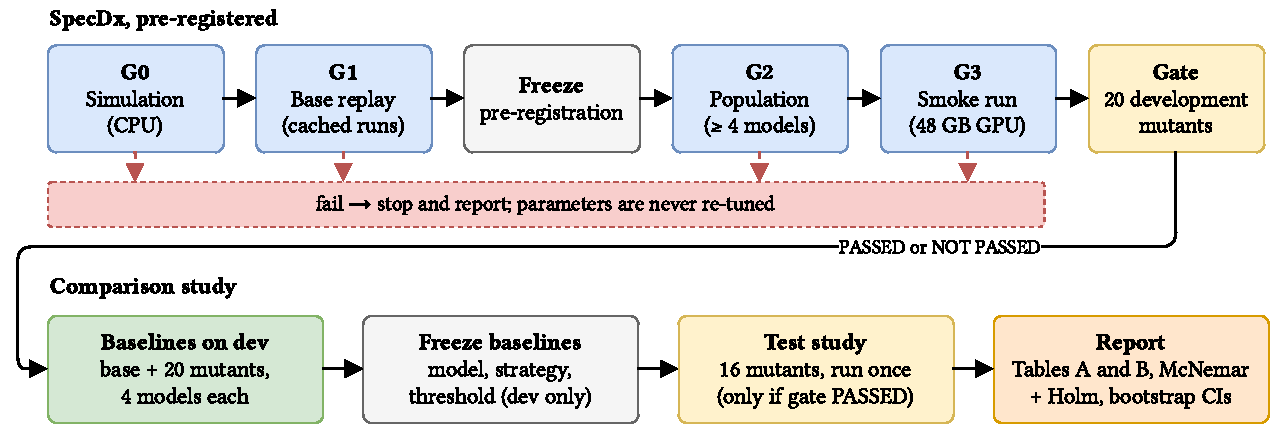
\includegraphics[width=\textwidth]{figures/drawio/protocol.pdf}
\caption{Evaluation protocol. Every go/no-go step has a pass criterion fixed in advance; a failure stops the study without re-tuning. The baselines are tuned on the development split whatever the gate's verdict, but the test split is run once, and only after the gate has passed and the baseline choices are frozen.}
\label{fig:protocol}
\end{figure}

\paragraph{G0: simulation.} We generate synthetic specifications with the following ingredients:
\begin{itemize}[leftmargin=*]
\item value and constraint cells, anchored and unanchored;
\item $M\in\{2,3,4\}$ models;
\item grouped difficulties, with an arm that spreads difficulty within groups;
\item Dirichlet errors, including concentrated ones;
\item planted defects of every form;
\item readings from three variants and three seeds, pooled over scenarios, with per-model act rates.
\end{itemize}
The generator is calibrated to summary statistics of base runs only, never to a mutant. The calibrated statistics are per-cell accuracy, dispersion, error concentration, act rates and readings per cell. Two \emph{misspecification arms} violate (A3), with model-specific errors, and (A5), with model-dependent silence.

The free parameters are chosen by a fixed rule: maximise mean simulated typed $F_1$ over hidden requirements, ambiguities and weak checks, at the calibrated point and the two arms with equal weight. Ties go to the more conservative setting.

G0 passes when all three criteria hold:
\begin{enumerate}[leftmargin=*,label=(\roman*)]
\item the mean $|\hat\theta_m-\theta_m|\le0.05$;
\item simulated typed $F_1\ge0.6$ for hidden requirements and $\ge0.4$ for ambiguity;
\item \specdx is never more than $0.05$ below the best simple baseline on any type, at the calibrated point, under either arm, and at the population's own size and accuracy gap; and it beats that baseline on ambiguity by more than $0.05$ at the calibrated point.
\end{enumerate}
The simple baselines are majority vote over models, ``deviates from the anchor'', and our earlier joint-class latent model. The regime map crosses mean cell accuracy $\{0.6,0.7,0.8,0.9,0.95\}$ with accuracy gap $\{0,0.1,0.2\}$ and $M\in\{2,4\}$, with at least five replicates per point and ten at the calibrated point.

\paragraph{G1: base replay.} The frozen model is fitted on cached base runs. It must not collapse: $\theta_m\ge0.5$ for the two strongest models. It must also report R-SO as a hidden requirement whenever the cell is observable.

\paragraph{G2: population.} The screen must admit at least four acting models from at least two families.

\paragraph{G3: smoke.} The base specification runs on the GPU host with a budget of 60, and every model must reach $\theta_m\ge0.5$.

\paragraph{Development gate.} On the 20 development mutants, \specdx wins a type under two rules:
\begin{itemize}[leftmargin=*]
\item \textbf{Contradiction and hidden requirement:} its typed $F_1$ exceeds the \emph{untyped} $F_1$ of both B2-naive and B3-2PL. These baselines cannot assign types, so a typed comparison would be trivially won.
\item \textbf{Ambiguity and weak check:} its typed $F_1$ is at least $0.4$. These baselines cannot locate truths in $\Tell$ or in fields at all.
\end{itemize}
A type with fewer than three scorable mutants counts as a loss, and the gate passes with at least three wins out of four. The test split stays locked until the gate passes.

\subsection{Statistics}

Comparisons are paired per mutant. We use the exact McNemar test on typed detection, comparing \specdx with each baseline, with Holm correction across baselines, and report paired risk differences as effect sizes. Confidence intervals are 95\% bootstrap intervals over mutants, with 10{,}000 resamples and a fixed seed. Because the test split is small, we emphasise effect sizes and intervals over $p$-values.

\subsection{Implementation and environment}

\specdx is implemented in Python 3.13. Inference uses NumPy. Hitting sets use PySAT~\cite{ignatiev2018pysat}, and the truth-inference baselines use crowd-kit~\cite{ustalov2024learning}. The implementation has an extensive unit and integration test suite. Every run is cached in an append-only log, keyed by the specification, the scenario, the interpreter and the model's weight digest, so that every table can be regenerated from raw logs.

Simulation, G0 and G1 run on a CPU. Interpreter runs use a single 48\,GB GPU with Ollama 0.30.4 and two parallel workers.

\section{Results}
\label{sec:results}

% NOTE TO AUTHORS: every number in this section is a placeholder (\tbd). The tables and
% figures are laid out for the final results; fill them from results/*.json and
% results/p3-report.md once the corresponding step has run.

\Cref{tab:gosteps} records the outcome of the pre-registered go/no-go steps. The results below are reported in the order of the research questions.

\begin{table}[t]
\caption{Outcome of the pre-registered go/no-go steps (\cref{sec:eval-sim}).}
\label{tab:gosteps}
\small
\begin{tabular}{@{}llll@{}}
\toprule
Step & Criterion & Measured & Outcome \\
\midrule
G0 & (i) mean $|\hat\theta-\theta|\le0.05$ & \tbd & \tbd \\
   & (ii) hidden $F_1\ge0.6$; ambiguity $F_1\ge0.4$ & \tbd\,/\,\tbd & \tbd \\
   & (iii) regime criteria (four points, three types) & \tbd & \tbd \\
G1 & no collapse; R-SO typed hidden if observable & \tbd & \tbd \\
G2 & $\ge4$ acting models, $\ge2$ families & \tbd & \tbd \\
G3 & smoke checks; $\theta_m\ge0.5$ for every model & \tbd & \tbd \\
Gate & $\ge3$ wins of 4 on the development split & \tbd & \tbd \\
\bottomrule
\end{tabular}
\end{table}

%-------------------------------------------------------------------------------------------
\subsection{RQ1: Identifiability in practice}
\label{sec:results-rq1}

\Cref{tab:sim} reports accuracy recovery and simulated typed $F_1$ at the calibrated point and under the two misspecification arms. \Cref{fig:regime} shows the regime map, and \cref{fig:sim-n} shows how $F_1$ grows with the number of readings per model and cell.

\begin{table}[t]
\caption{Simulation at the calibrated point and under the misspecification arms. Typed $F_1$ (mean over replicates, with 95\% interval). Contradictions are symbolic and are not simulated.}
\label{tab:sim}
\small
\begin{tabular}{@{}l ccc ccc ccc@{}}
\toprule
 & \multicolumn{3}{c}{Calibrated} & \multicolumn{3}{c}{(A3) violated} & \multicolumn{3}{c}{(A5) violated} \\
\cmidrule(lr){2-4}\cmidrule(lr){5-7}\cmidrule(l){8-10}
Method & Hid. & Amb. & Weak & Hid. & Amb. & Weak & Hid. & Amb. & Weak \\
\midrule
\specdx (anchored cell model) & \tbd & \tbd & \tbd & \tbd & \tbd & \tbd & \tbd & \tbd & \tbd \\
Majority vote over models & \tbd & \tbd & \tbd & \tbd & \tbd & \tbd & \tbd & \tbd & \tbd \\
Deviates from anchor & \tbd & \tbd & \tbd & \tbd & \tbd & \tbd & \tbd & \tbd & \tbd \\
Joint-class latent model & \tbd & \tbd & \tbd & \tbd & \tbd & \tbd & \tbd & \tbd & \tbd \\
\midrule
\multicolumn{10}{@{}l}{Mean accuracy error $|\hat\theta_m-\theta_m|$ of \specdx: \tbd\ (calibrated), \tbd\ (A3), \tbd\ (A5); non-converged fits: \tbd} \\
\bottomrule
\end{tabular}
\end{table}

\begin{figure}[t]
\centering
\newcommand{\regimepanel}[3]{%
  \begin{scope}[shift={(#1)}]
    \node[font=\scriptsize\bfseries, anchor=south] at (1.25,1.65) {#2};
    \foreach \i in {0,...,4} {\foreach \j in {0,1,2} {
      \draw[gray!60, fill=white] (\i*0.5,\j*0.5) rectangle ++(0.5,0.5);
      \node[font=\tiny, gray] at (\i*0.5+0.25,\j*0.5+0.25) {--};
    }}
    \foreach \a [count=\i from 0] in {.6,.7,.8,.9,.95} {\node[font=\tiny, anchor=north] at (\i*0.5+0.25,0) {\a};}
    #3
  \end{scope}}
\begin{tikzpicture}
  \regimepanel{0,2.7}{Hidden, $M=2$}{\foreach \d [count=\j from 0] in {0,.1,.2} {\node[font=\tiny, anchor=east] at (0,\j*0.5+0.25) {\d};}\node[font=\scriptsize, rotate=90] at (-0.55,0.75) {gap $\Delta$};}
  \regimepanel{3.2,2.7}{Ambiguity, $M=2$}{}
  \regimepanel{6.4,2.7}{Weak, $M=2$}{}
  \regimepanel{0,0}{Hidden, $M=4$}{\foreach \d [count=\j from 0] in {0,.1,.2} {\node[font=\tiny, anchor=east] at (0,\j*0.5+0.25) {\d};}\node[font=\scriptsize, rotate=90] at (-0.55,0.75) {gap $\Delta$};}
  \regimepanel{3.2,0}{Ambiguity, $M=4$}{}
  \regimepanel{6.4,0}{Weak, $M=4$}{}
  \node[font=\scriptsize] at (4.45,-0.6) {mean cell accuracy};
  \begin{scope}[shift={(9.6,0.6)}, font=\scriptsize]
    \draw[fill=green!45] (0,1.6) rectangle ++(0.3,0.3); \node[anchor=west] at (0.35,1.75) {win};
    \draw[fill=gray!25]  (0,1.0) rectangle ++(0.3,0.3); \node[anchor=west] at (0.35,1.15) {tie};
    \draw[fill=red!40]   (0,0.4) rectangle ++(0.3,0.3); \node[anchor=west] at (0.35,0.55) {loss};
  \end{scope}
\end{tikzpicture}
\caption{Regime map: \specdx against the best simple baseline in each cell of the simulation grid (margin $0.05$; at least five replicates per cell). Cells will be coloured win, tie or loss. The boundaries predicted by \cref{thm:t2,thm:t2prime,thm:t4} are to be overlaid.}
\label{fig:regime}
\end{figure}

\begin{figure}[t]
\centering
\begin{tikzpicture}
\begin{groupplot}[
  group style={group size=3 by 1, horizontal sep=10mm, y descriptions at=edge left},
  width=0.36\textwidth, height=0.28\textwidth,
  xmin=0, xmax=40, ymin=0, ymax=1,
  xlabel={readings per model and cell $n$}, ylabel={typed $F_1$},
  xtick={0,10,20,30,40}, ytick={0,0.2,0.4,0.6,0.8,1},
  tick label style={font=\scriptsize}, label style={font=\scriptsize}, title style={font=\footnotesize},
  legend style={font=\scriptsize, draw=none, legend columns=4, at={(-0.75,-0.42)}, anchor=north}]
\nextgroupplot[title={Hidden requirement}]
\nextgroupplot[title={Ambiguity}]
\nextgroupplot[title={Weak check}]
  \addlegendimage{black, thick, mark=*}\addlegendentry{\specdx}
  \addlegendimage{blue, thick, dashed, mark=square*}\addlegendentry{majority vote}
  \addlegendimage{red, thick, dotted, mark=triangle*}\addlegendentry{deviates from anchor}
  \addlegendimage{gray, thick, dashdotted, mark=diamond*}\addlegendentry{joint-class model}
\end{groupplot}
\end{tikzpicture}
\caption{Simulated typed $F_1$ against the number of readings per model and cell, at the calibrated point. Data to be added.}
\label{fig:sim-n}
\end{figure}

\paragraph{Accuracy recovery.} [To be written: how closely $\hat\theta_m$ tracks the true accuracy, and whether the multi-start EM avoids the collapse of the earlier model.]

\paragraph{Typing.} [To be written: typed $F_1$ against the simple baselines at the calibrated point; the effect of the (A3) and (A5) arms.]

\paragraph{Calibration.} \Cref{fig:calibration} compares the posterior defect probabilities with the observed frequency of planted defects. [To be written.]

\begin{figure}[t]
\centering
\begin{tikzpicture}
\begin{groupplot}[
  group style={group size=3 by 1, horizontal sep=10mm, y descriptions at=edge left},
  width=0.36\textwidth, height=0.36\textwidth,
  xmin=0, xmax=1, ymin=0, ymax=1,
  xlabel={posterior probability}, ylabel={observed frequency},
  xtick={0,0.25,0.5,0.75,1}, ytick={0,0.25,0.5,0.75,1},
  tick label style={font=\scriptsize}, label style={font=\scriptsize}, title style={font=\footnotesize},
  legend style={font=\scriptsize, draw=none, legend columns=3, at={(-0.75,-0.38)}, anchor=north}]
\nextgroupplot[title={$\Prob(A_c\neq\{d_c\})$ (hidden)}]
  \addplot[gray, dashed, domain=0:1] {x};
\nextgroupplot[title={$\Prob(|A_c|=2)$ (ambiguity)}]
  \addplot[gray, dashed, domain=0:1] {x};
\nextgroupplot[title={MAP posterior (weak check)}]
  \addplot[gray, dashed, domain=0:1] {x};
  \addlegendimage{black, thick, mark=*}\addlegendentry{calibrated point}
  \addlegendimage{blue, thick, dashed, mark=square*}\addlegendentry{(A3) violated}
  \addlegendimage{red, thick, dotted, mark=triangle*}\addlegendentry{(A5) violated}
\end{groupplot}
\end{tikzpicture}
\caption{Calibration of the posterior defect probabilities in simulation (reliability diagrams, ten bins). The dashed diagonal is perfect calibration. Data to be added.}
\label{fig:calibration}
\end{figure}

\paragraph{Regimes.} [To be written: where \specdx wins, ties or loses; agreement of the empirical boundaries with \cref{thm:t2,thm:t2prime,thm:t4}.]

\rqanswer{1}{[To be completed once the results are final.]}

%-------------------------------------------------------------------------------------------
\subsection{RQ2: Effectiveness on seeded defects}
\label{sec:results-rq2}

\Cref{tab:main} gives typed $F_1$ per defect type, average precision and Detection@$k$ on the scorable mutants of the test split. Every method runs at its native protocol (Table A). \Cref{tab:paired} gives the paired comparisons, and \cref{fig:f1bars} shows typed $F_1$ by type. The corresponding tables for all mutants and for the development split are in the supplementary material.

\begin{table}[t]
\caption{Table A: effectiveness on scorable test mutants, every method at its native protocol. Typed $F_1$ per type; mean AP and Detection@$k$ over types the method reports; cost in model requests. ``\nr'' marks a type the method does not report. Scorable mutants per type: \tbd\,/\,\tbd\,/\,\tbd\,/\,\tbd.}
\label{tab:main}
\small
\setlength{\tabcolsep}{4.5pt}
\begin{tabular}{@{}l cccc c ccc r@{}}
\toprule
 & \multicolumn{4}{c}{Typed $F_1$} & & \multicolumn{3}{c}{Detection@$k$} & \\
\cmidrule(lr){2-5}\cmidrule(lr){7-9}
Method & Con. & Hid. & Amb. & Weak & AP & 1 & 3 & 5 & Requests \\
\midrule
\specdx & \tbd & \tbd & \tbd & \tbd & \tbd & \tbd & \tbd & \tbd & \tbd \\
\midrule
B1 BenchGuard & \tbd & \tbd & \tbd & \tbd & \tbd & \tbd & \tbd & \tbd & \tbd \\
B2 Who\&When & \nr & \tbd & \nr & \nr & \tbd & \tbd & \tbd & \tbd & \tbd \\
B3 IRT audit & \nr & \tbd & \nr & \nr & \tbd & \tbd & \tbd & \tbd & \tbd \\
B4 Semantic entropy & \nr & \nr & \tbd & \nr & \tbd & \tbd & \tbd & \tbd & \tbd \\
B5 MUS on $\Chk$ & \tbd & \nr & \nr & \nr & \tbd & \tbd & \tbd & \tbd & \tbd \\
TI GLAD & \nr & \tbd & \nr & \nr & \tbd & \tbd & \tbd & \tbd & \tbd \\
TI Dawid--Skene & \nr & \tbd & \nr & \nr & \tbd & \tbd & \tbd & \tbd & \tbd \\
JEST & \nr & \tbd & \nr & \nr & \tbd & \tbd & \tbd & \tbd & \tbd \\
\midrule
B2-naive & \nr & \tbd & \nr & \nr & \tbd & \tbd & \tbd & \tbd & \tbd \\
B3-2PL & \nr & \tbd & \nr & \nr & \tbd & \tbd & \tbd & \tbd & \tbd \\
\bottomrule
\end{tabular}
\end{table}

\begin{table}[t]
\caption{Paired comparison on typed detection (scorable test mutants): risk difference \specdx $-$ baseline with 95\% bootstrap interval, and exact McNemar $p$-value after Holm correction. Only types the baseline reports are compared.}
\label{tab:paired}
\small
\begin{tabular}{@{}l l c c@{}}
\toprule
Baseline & Type & Risk difference [95\% CI] & $p_{\text{Holm}}$ \\
\midrule
B1 BenchGuard & each of four & \tbd\ [\tbd, \tbd] & \tbd \\
B2 Who\&When & \Dhid & \tbd\ [\tbd, \tbd] & \tbd \\
B3 IRT audit & \Dhid & \tbd\ [\tbd, \tbd] & \tbd \\
B4 Semantic entropy & \Damb & \tbd\ [\tbd, \tbd] & \tbd \\
B5 MUS on $\Chk$ & \Dcon & \tbd\ [\tbd, \tbd] & \tbd \\
TI (best of GLAD, DS) & \Dhid & \tbd\ [\tbd, \tbd] & \tbd \\
JEST & \Dhid & \tbd\ [\tbd, \tbd] & \tbd \\
\bottomrule
\end{tabular}
\end{table}

\begin{figure}[t]
\centering
\begin{tikzpicture}
\begin{axis}[
  width=0.92\textwidth, height=0.3\textwidth,
  ybar, bar width=4pt, ymin=0, ymax=1, xmin=0.5, xmax=4.5,
  xtick={1,2,3,4}, xticklabels={Contradiction, Hidden requirement, Ambiguity, Weak check},
  ylabel={typed $F_1$}, ytick={0,0.2,0.4,0.6,0.8,1},
  tick label style={font=\scriptsize}, label style={font=\scriptsize},
  ymajorgrids, grid style={gray!20},
  legend style={font=\scriptsize, draw=none, legend columns=8, at={(0.5,1.03)}, anchor=south, /tikz/every even column/.append style={column sep=3mm}},
  extra y ticks={0.4}, extra y tick style={grid=major, major grid style={red, dashed}}, extra y tick labels={}]
  \addlegendimage{ybar, ybar legend, fill=black}\addlegendentry{\specdx}
  \addlegendimage{ybar, ybar legend, fill=blue!60}\addlegendentry{B1}
  \addlegendimage{ybar, ybar legend, fill=cyan!50}\addlegendentry{B2}
  \addlegendimage{ybar, ybar legend, fill=teal!50}\addlegendentry{B3}
  \addlegendimage{ybar, ybar legend, fill=orange!60}\addlegendentry{B4}
  \addlegendimage{ybar, ybar legend, fill=violet!50}\addlegendentry{B5}
  \addlegendimage{ybar, ybar legend, fill=gray!50}\addlegendentry{TI}
  \addlegendimage{ybar, ybar legend, fill=brown!50}\addlegendentry{JEST}
\end{axis}
\end{tikzpicture}
\caption{Typed $F_1$ by defect type on scorable test mutants, with 95\% bootstrap intervals. The dashed line marks the $0.4$ bar of the development gate for ambiguity and weak checks. Data to be added.}
\label{fig:f1bars}
\end{figure}

\paragraph{Contradictions.} [To be written.]

\paragraph{Hidden requirements.} [To be written.]

\paragraph{Ambiguities and localisation.} [To be written, including the share of ambiguities that ddmin localised and the size of the reported sentence sets.]

\paragraph{Weak checks.} [To be written.]

\paragraph{False positives on the base specification.} \Cref{fig:base-findings} shows the findings each method reports on the unmutated base specification. [To be written: the number of findings by type, and how many fall on the Unobservable list.]

\begin{figure}[t]
\centering
\begin{tikzpicture}
\begin{axis}[
  width=0.92\textwidth, height=0.3\textwidth,
  ybar stacked, bar width=10pt, ymin=0, ymax=100, xmin=0.4, xmax=8.6,
  xtick={1,...,8}, xticklabels={\specdx, B1, B2, B3, B4, B5, TI, JEST},
  ylabel={findings on the base}, tick label style={font=\scriptsize}, label style={font=\scriptsize},
  ymajorgrids, grid style={gray!20},
  legend style={font=\scriptsize, draw=none, legend columns=5, at={(0.5,1.03)}, anchor=south},
  /tikz/every even column/.append style={column sep=3mm}]
  \addlegendimage{ybar, ybar legend, fill=purple!40}\addlegendentry{\Dcon}
  \addlegendimage{ybar, ybar legend, fill=red!40}\addlegendentry{\Dhid}
  \addlegendimage{ybar, ybar legend, fill=yellow!60}\addlegendentry{\Damb}
  \addlegendimage{ybar, ybar legend, fill=green!40}\addlegendentry{\Dweak}
  \addlegendimage{ybar, ybar legend, fill=gray!25}\addlegendentry{Unobservable (not scored)}
\end{axis}
\end{tikzpicture}
\caption{Findings on the unmutated base specification, by type. Real defects among them are counted in \cref{sec:results-rq3}; the rest are candidate false positives. The y-axis range is a placeholder. Data to be added.}
\label{fig:base-findings}
\end{figure}

\rqanswer{2}{[To be completed once the results are final.]}

%-------------------------------------------------------------------------------------------
\subsection{RQ3: Real defects}
\label{sec:results-rq3}

\Cref{tab:real-results} reports, for each real defect, whether each method reports it with the right type and location, at what rank, and after how many population runs.

\begin{table}[t]
\caption{Real defects. \checkmark: reported with matching type and location; $\circ$: reported untyped or mislocated; $\times$: not reported; ``unobs.'': not observable by the population. Rank among the method's findings and population runs until first report (\specdx only).}
\label{tab:real-results}
\small
\begin{tabular}{@{}l ccc ccccccc@{}}
\toprule
 & \multicolumn{3}{c}{\specdx} & & & & & & & \\
\cmidrule(lr){2-4}
Defect & Found & Rank & Runs & B1 & B2 & B3 & B4 & B5 & TI & JEST \\
\midrule
R-SO (\Dhid) & \tbd & \tbd & \tbd & \tbd & \tbd & \tbd & \nr & \nr & \tbd & \tbd \\
R-12 (\Dcon) & \tbd & \tbd & \tbd & \tbd & \nr & \nr & \nr & \tbd & \nr & \nr \\
R-DE (\Dhid) & \tbd & \tbd & \tbd & \tbd & \tbd & \tbd & \nr & \nr & \tbd & \tbd \\
\bottomrule
\end{tabular}
\end{table}

\Cref{fig:rso} looks inside the anchored cell model at the R-SO cell: the share of readings that move away from the anchor for each model, and the posterior over the cell's candidate sets.

\begin{figure}[t]
\centering
\begin{tikzpicture}
\begin{groupplot}[
  group style={group size=2 by 1, horizontal sep=16mm},
  width=0.46\textwidth, height=0.32\textwidth,
  tick label style={font=\scriptsize}, label style={font=\scriptsize}, title style={font=\footnotesize}]
\nextgroupplot[title={(a) readings by model}, ybar stacked, bar width=12pt, ymin=0, ymax=1, xmin=0.4, xmax=4.6,
  xtick={1,...,4}, xticklabels={model 1, model 2, model 3, model 4}, ylabel={share of acted readings},
  xlabel={models ordered by $\hat\theta_m$},
  legend style={font=\scriptsize, draw=none, at={(0.5,-0.42)}, anchor=north, legend columns=3}]
  \addlegendimage{ybar, ybar legend, fill=orange!40}\addlegendentry{\vi{Chờ duyệt} ($d_c$)}
  \addlegendimage{ybar, ybar legend, fill=green!40}\addlegendentry{\vi{Đã duyệt}}
  \addlegendimage{ybar, ybar legend, fill=gray!30}\addlegendentry{other}
\nextgroupplot[title={(b) posterior over $A_c$}, ybar, bar width=12pt, ymin=0, ymax=1, xmin=0.4, xmax=5.6,
  xtick={1,...,5}, xticklabels={{$\{d_c\}$}, {\{\vi{Đã}\}}, {$\{d_c$, \vi{Đã}$\}$}, {$\emptyset$}, {other}},
  ylabel={posterior probability}, extra y ticks={0.5}, extra y tick style={grid=major, major grid style={red, dashed}}, extra y tick labels={}]
\end{groupplot}
\end{tikzpicture}
\caption{Inside the diagnosis of R-SO. (a)~For each model, the share of its acted readings of the cell \texttt{SO-0031}.status that equal the anchor, the alternative reading, or something else. (b)~The posterior over the cell's candidate sets; the dashed line marks $\tau_H$. Data to be added.}
\label{fig:rso}
\end{figure}

[To be written: discussion of each real defect, including the witness that \specdx reports and, for R-12, the synthesised scenario that exposed it. R-DOC is discussed qualitatively for B1.]

\rqanswer{3}{[To be completed once the results are final.]}

%-------------------------------------------------------------------------------------------
\subsection{RQ4: Cost-effectiveness}
\label{sec:results-rq4}

\Cref{fig:anytime} shows the detection rate of \specdx at its anytime checkpoints, together with the native cost of each baseline. \Cref{tab:equalcost} compares each LLM-based baseline with \specdx at equal cost (Table B).

\begin{figure}[t]
\centering
\begin{tikzpicture}
\begin{axis}[
  width=0.62\textwidth, height=0.36\textwidth,
  xmin=0, xmax=210, ymin=0, ymax=1,
  xtick={0,25,50,100,150,200}, ytick={0,0.2,0.4,0.6,0.8,1},
  xlabel={population runs}, ylabel={typed detection rate},
  tick label style={font=\scriptsize}, label style={font=\scriptsize},
  xmajorgrids, grid style={gray!20},
  legend style={font=\scriptsize, draw=none, at={(1.03,0.5)}, anchor=west}]
  \addlegendimage{black, thick, mark=*}\addlegendentry{\specdx (all types)}
  \addlegendimage{black, thick, dashed, mark=o}\addlegendentry{\specdx, X9: random scenarios}
  \addlegendimage{black, thick, dotted, mark=square}\addlegendentry{\specdx, X13: no escalation}
  \addlegendimage{only marks, mark=triangle*, blue}\addlegendentry{B1 at its native cost}
  \addlegendimage{only marks, mark=diamond*, cyan}\addlegendentry{B2 at its native cost}
\end{axis}
\end{tikzpicture}
\caption{Anytime behaviour: typed detection rate of \specdx at the checkpoints of 25, 50, 100, 150 and 200 population runs, with two ablations of the scenario policy. Ambiguities count as detected only at the final checkpoint, because localisation runs last. Data to be added.}
\label{fig:anytime}
\end{figure}

\begin{table}[t]
\caption{Table B: equal cost. Each LLM-based baseline at its native protocol, against \specdx at the checkpoint whose cost is closest to, and not above, the baseline's.}
\label{tab:equalcost}
\small
\begin{tabular}{@{}l r r cccc@{}}
\toprule
 & & \specdx & \multicolumn{4}{c}{Typed $F_1$ (baseline\,/\,\specdx)} \\
\cmidrule(l){4-7}
Baseline & Requests & checkpoint & Con. & Hid. & Amb. & Weak \\
\midrule
B1 BenchGuard & \tbd & \tbd & \tbd\,/\,\tbd & \tbd\,/\,\tbd & \tbd\,/\,\tbd & \tbd\,/\,\tbd \\
B2 Who\&When & \tbd & \tbd & \nr\,/\,\tbd & \tbd\,/\,\tbd & \nr\,/\,\tbd & \nr\,/\,\tbd \\
\bottomrule
\end{tabular}
\end{table}

\Cref{fig:cost} breaks the cost of each method down by what the requests were spent on.

\begin{figure}[t]
\centering
\begin{tikzpicture}
\begin{axis}[
  width=0.92\textwidth, height=0.3\textwidth,
  xbar stacked, bar width=8pt, xmin=0, xmax=1000, ymin=0.4, ymax=8.6,
  ytick={1,...,8}, yticklabels={\specdx, B1 BenchGuard, B2 Who\&When, B3 IRT audit, B4 Sem.\ entropy, B5 MUS on $\Chk$, TI, JEST},
  y dir=reverse, xlabel={model requests per specification},
  tick label style={font=\scriptsize}, label style={font=\scriptsize}, xmajorgrids, grid style={gray!20},
  legend style={font=\scriptsize, draw=none, legend columns=5, at={(0.5,1.03)}, anchor=south},
  /tikz/every even column/.append style={column sep=3mm}]
  \addplot[draw=none, forget plot] coordinates {(0,0.4) (0,8.6)};
  \addlegendimage{xbar, xbar legend, fill=blue!40}\addlegendentry{population runs}
  \addlegendimage{xbar, xbar legend, fill=purple!40}\addlegendentry{refutation probes}
  \addlegendimage{xbar, xbar legend, fill=yellow!60}\addlegendentry{ddmin tests}
  \addlegendimage{xbar, xbar legend, fill=orange!50}\addlegendentry{own LLM calls}
\end{axis}
\end{tikzpicture}
\caption{Cost per specification in model requests, by component. Baselines that consume \specdx's runs are charged those runs plus their own calls. The x-axis range is a placeholder. Data to be added.}
\label{fig:cost}
\end{figure}

[To be written: runs to first detection per type; the share of scenarios escalated; the cost of refutation and localisation relative to population runs; wall-clock time on the 48\,GB GPU.]

\rqanswer{4}{[To be completed once the results are final.]}

%-------------------------------------------------------------------------------------------
\subsection{RQ5: Ablation}
\label{sec:results-rq5}

\Cref{tab:ablation} reports the change in typed $F_1$ when one component is removed or replaced.

\begin{table}[t]
\caption{Ablation on the scorable mutants: change in typed $F_1$ relative to full \specdx (negative means the component helps).}
\label{tab:ablation}
\small
\begin{tabular}{@{}llcccc@{}}
\toprule
Id & Variant & Con. & Hid. & Amb. & Weak \\
\midrule
--  & Full \specdx (typed $F_1$) & \tbd & \tbd & \tbd & \tbd \\
\midrule
X1 & No anchor: latent truth without $d_c$ in the prior & \tbd & \tbd & \tbd & \tbd \\
X2 & Joint class over a whole step instead of cells & \tbd & \tbd & \tbd & \tbd \\
X3 & Free per-cell $\varepsilon_c$ instead of the flat pool & \tbd & \tbd & \tbd & \tbd \\
X4 & Per-cell instead of grouped difficulty & \tbd & \tbd & \tbd & \tbd \\
X5 & Single-truth Dawid--Skene instead of set-valued $A_c$ & \tbd & \tbd & \tbd & \tbd \\
X6 & No stage 1 (no observability gating) & \tbd & \tbd & \tbd & \tbd \\
X7 & Single-clause tests only (no hitting-set duality) & \tbd & \tbd & \tbd & \tbd \\
X8 & No refutation & \tbd & \tbd & \tbd & \tbd \\
X9 & Random scenarios instead of Thompson sampling & \tbd & \tbd & \tbd & \tbd \\
X10 & No T-boundary scenarios & \tbd & \tbd & \tbd & \tbd \\
X11 & Lexical-overlap localisation instead of ddmin & \tbd & \tbd & \tbd & \tbd \\
X12 & Two models instead of four & \tbd & \tbd & \tbd & \tbd \\
X13 & No escalation: always run the full population & \tbd & \tbd & \tbd & \tbd \\
\bottomrule
\end{tabular}
\end{table}

[To be written.]

\rqanswer{5}{[To be completed once the results are final.]}

\section{Discussion}
\label{sec:discussion}

% NOTE TO AUTHORS: the paragraphs below discuss the design. Sentences that depend on the
% final numbers are marked [..] and should be revised once the results are in.

\subsection{What the population buys}

A natural question is why \specdx runs many weak readers instead of asking one strong reviewer. The theory gives a precise answer: a single reader can only separate a defect from an error through a plurality margin (\cref{thm:t1}). Such a margin does not exist exactly where specifications are hardest, at cells that most readers get wrong for reasons of their own. A population buys two things that a single reviewer cannot provide.
\begin{itemize}[leftmargin=*]
\item \textbf{An accuracy gradient.} With it, the direction in which each reading moves as competence grows becomes evidence in its own right (\cref{lem:signatures}). The second reading of an ambiguous cell rises with competence, while a concentrated error falls, even if the two have the same frequency.
\item \textbf{Anchored contrasts.} These rank the readers without any human label, provided most anchors are right (\cref{thm:t3}).
\end{itemize}
The design has a consequence: the readers do not need to be strong. They need to be \emph{different} in competence, to act often enough to be observed, and to agree with the anchor on most cells. This is why the capability screen measures acting, not agreement with $\Chk$, and why mid-sized local models suffice. [Revise with the RQ5 result for two models against four.]

\subsection{Implications for specification authors}

\specdx reports each defect with three pieces of evidence that an author can check directly:
\begin{itemize}[leftmargin=*]
\item a location in the artefact the author edits: a clause, a field, or a set of sentences;
\item a witness: a state that satisfies the remaining clauses, or a run that passes every check while the population disagrees with it;
\item a posterior that says how sure the method is.
\end{itemize}
Each type points to a different repair. A hidden requirement asks the author either to state the rule in $\Tell$ or to relax the clause. An ambiguity asks for the sentences returned by ddmin to be sharpened. A weak check asks for a clause on the reported field. A contradiction asks the author to decide which of the conflicting clauses is wrong. We expect the unstated subtype to be common in golden states: rows that the reference run happened to write, but that no sentence of $\Tell$ asks for. [Revise with RQ3 and the base-specification findings.]

\subsection{Implications for benchmark builders}

Benchmarks for LLM agents are executable specifications in our sense. Several recent audits repaired them by hand~\cite{cuadron2025saber,zhu2025establishing,cao2026policy}. \specdx offers an automatic first pass that needs no frontier model and no labels, and that types its findings, so a maintainer can triage them. Two lessons from the design apply even without \specdx.
\begin{itemize}[leftmargin=*]
\item \textbf{A failing run is not evidence against the agent until competent agents also fail at the same place.} The anchored contrasts of \cref{thm:t3} are a cheap way to check this.
\item \textbf{A benchmark item that no agent reaches cannot be validated by running agents} (\cref{prop:noaction}). Audits should report such items separately instead of counting them as correct.
\end{itemize}

\subsection{Limits of the approach}

\paragraph{Defects outside behaviour.} \specdx finds only what some behaviour can expose. Documentation-only inconsistencies, such as a README that miscounts the invariants, are invisible to it by construction. Static review remains the right tool for them.

\paragraph{Regime dependence.} The anchored cell model beats simple aggregators only in some regimes. Majority vote is as good when accuracy is moderate and the population is small, and flagging every deviation from the anchor is as good on hidden requirements, though it cannot see ambiguity. We report the whole regime map (\cref{fig:regime}) instead of a single operating point, so that a user can tell from the screen statistics of their own population whether the extra machinery is worth it.

\paragraph{Weak checks remain hard.} A weak check is witnessed only by a behaviour that $\Tell$ forbids. \specdx therefore depends on interpreters making the \emph{right} mistakes at the unguarded field, while still being competent elsewhere. In simulation, this was the type whose performance depended most on generator assumptions that the base data do not determine. We therefore treated simulated weak-check $F_1$ as information only. [Revise with the RQ2 result.]

\paragraph{Contradictions are only refuted, never proven.} A reported contradiction means that neither the population nor the symbolic repair found a satisfying state within budget. The report says how hard the search tried. A complete check would need an encoding of $\Chk$ that a solver can decide. For procedural SQL such as \texttt{fn\_reconcile}, building one is a project in itself.

\paragraph{Cost.} A full diagnosis costs at most 380 runs of a multi-step process. On a single 48\,GB GPU this is [hours/days, to be measured]. The cache makes re-diagnosis after an edit cheap, because only runs whose inputs changed are repeated. The pilot-then-escalate policy keeps uninformative scenarios cheap. [Revise with RQ4.]

\subsection{Beyond procure-to-pay}

Nothing in the model is specific to procurement or to Vietnamese. The ingredients are only these:
\begin{itemize}[leftmargin=*]
\item a text that executors read;
\item checks that can be evaluated on an end state;
\item a way to vary scenarios.
\end{itemize}
$\tau^2$-bench~\cite{barres2026bench} fits this mould: its policy document is $\Tell$, and its expected actions and database fields are $\Chk$. The repairs of its verified release give real defects with types. We have designed but not yet built this second subject. Its tasks are fixed, so scenario synthesis does not apply, and its user simulator adds a source of variation that the model would have to absorb. Business-process settings with executable process models and conformance checks~\cite{fahland2015model,calvanese2026agentic} are another natural target.

\section{Threats to Validity}
\label{sec:threats}

\paragraph{Construct validity.}
\begin{itemize}[leftmargin=*]
\item \textbf{Seeded defects may not resemble real ones.} We mitigate this in three ways. The operators are derived from defect categories that published benchmark audits report~\cite{cuadron2025saber,zhu2025establishing}. Every mutant carries a kill witness, so none is equivalent. We also evaluate on real defects from the subject's history.
\item \textbf{The matching rules decide what counts as a detection.} The rules were fixed before any method ran, are the same for all methods, and are implemented once in shared scoring code.
\item \textbf{Scorability could look like cherry-picking.} The scorable set is computed from base runs only, before any mutant runs, and is identical for every method. Tables over all mutants are always reported alongside it.
\end{itemize}

\paragraph{Internal validity.}
\begin{itemize}[leftmargin=*]
\item \textbf{LLM errors are correlated across models.} This could make a shared misreading look like the truth. The anchored contrasts and the regime analysis address this, and the (A3) arm of the simulation measures the effect directly.
\item \textbf{Non-determinism.} We fix temperatures and seeds, pin model weight digests, fix the Ollama version, and cache every run with its digest.
\item \textbf{The Tell variants are generated by an LLM.} They paraphrase only the standing instruction and the task statement, and they were frozen once and are published.
\item \textbf{The hyper-parameters may be overfitted.} \specdx's thresholds were chosen by simulation calibrated to base runs only. The baselines' thresholds were chosen on the development split, which favours the baselines.
\item \textbf{The development gate is a second iteration on the same 20 development mutants.} An earlier version of the method was gated on them. The integrity rules of \cref{sec:eval-sim} limit the risk:
  \begin{itemize}
  \item every parameter of the current version was frozen before the gate;
  \item the development mutants are used once per version;
  \item the test split was never touched before the final study.
  \end{itemize}
\item \textbf{The population was relaxed after the screen.} The admission threshold on act rate was lowered from $0.6$ to $0.3$ during design, while the screen results were known. The screen reads no mutant and no truth, and the change was recorded in the pre-registration before any result of the current version.
\end{itemize}

\paragraph{External validity.}
\begin{itemize}[leftmargin=*]
\item \textbf{One subject.} The study covers one specification in one language and one domain.
\item \textbf{A narrow population.} It uses four local models of up to about 30B parameters from three families. Larger or hosted models might act more reliably and change the regime.
\item \textbf{Baselines on open models.} The LLM-based baselines B1 and B2 run on the same open models instead of the frontier models of their original papers, so their absolute performance may be lower than reported there. Each baseline's best model is selected on the development split, and the comparison at equal models is the fair one for our question.
\end{itemize}

\paragraph{Conclusion validity.}
\begin{itemize}[leftmargin=*]
\item \textbf{The test split is small.} The current operators yield 36 mutants, 16 of them in the test split. Two types have only two test mutants, so per-type McNemar tests have low power.
\item \textbf{Mitigations.} We report paired risk differences with bootstrap intervals and Holm-corrected exact tests, and we interpret effect sizes rather than $p$-values. Growing the operator sites is the most direct way to strengthen the conclusions, and we leave it to future work.
\end{itemize}

\section{Related Work}
\label{sec:related}

\specdx draws on several lines of work that rarely meet. \Cref{tab:positioning} summarises how it relates to the closest of them.

\begin{table}[t]
\caption{Positioning. \checkmark: the property holds; $\circ$: partially or in some variants; blank: it does not.}
\label{tab:positioning}
\footnotesize
\setlength{\tabcolsep}{2.5pt}
\resizebox{\textwidth}{!}{%
\begin{tabular}{@{}l ccccccc@{}}
\toprule
Approach & \makecell{Executes\\$\Tell$} & \makecell{Uses $\Chk$\\as evidence} & \makecell{Several\\models} & \makecell{Rater\\competence} & \makecell{Set-valued\\truth} & \makecell{Typed\\findings} & \makecell{Logical\\witness} \\
\midrule
LLM requirements review~\cite{fantechi2023inconsistency,gartner2024automated,hall2026neurosymbolic} & & & & & & $\circ$ & $\circ$ \\
LLM benchmark auditors~\cite{tu2026who,wang2026automated,suh2026agentsuite} & & \checkmark & & & & \checkmark & \\
Ambiguity by sampling~\cite{mu2024clarifygpt,jia2025automated} & \checkmark & & & & & & \\
$N{+}1$-version testing~\cite{park2021jest} & \checkmark & \checkmark & \checkmark & & & $\circ$ & \\
IRT audits~\cite{rodriguez2021evaluation,land2026auditing} & \checkmark & \checkmark & \checkmark & \checkmark & & & \\
Truth inference~\cite{dawid1979maximum,whitehill2009whose} & & & \checkmark & \checkmark & $\circ$ & & \\
Semantic entropy~\cite{kuhn2023semantic,farquhar2024detecting} & \checkmark & & $\circ$ & & & & \\
MUS / core extraction~\cite{liffiton2008algorithms,torlak2008finding} & & \checkmark & & & & $\circ$ & \checkmark \\
Failure attribution~\cite{zhang2025which,ge2026spectrum} & \checkmark & \checkmark & & & & $\circ$ & \\
\midrule
\specdx & \checkmark & \checkmark & \checkmark & \checkmark & \checkmark & \checkmark & \checkmark \\
\bottomrule
\end{tabular}}
\end{table}

\subsection{Validity of benchmarks and executable specifications}

A growing body of work shows that the checks of popular benchmarks are often wrong.
\begin{itemize}[leftmargin=*]
\item \textbf{Code benchmarks.} Test-based evaluation of code misses many wrong programs~\cite{liu2023your}. In SWE-bench, a substantial fraction of patches that pass the tests are incorrect or exploit weak tests~\cite{wang2026solved,yu2025utboost,yu2026swe}.
\item \textbf{Agent benchmarks.} Annotation errors and underspecified tasks have been reported in $\tau$-bench~\cite{cuadron2025saber} and in many agentic benchmarks under a common checklist~\cite{zhu2025establishing}. Others have been found in tool-calling evaluations~\cite{bhat2026benchmarking} and data-engineering benchmarks~\cite{zanoli2026elt}. Cao et al.\ show that policy ambiguity often masquerades as agent error~\cite{cao2026policy}.
\item \textbf{Label errors.} Even well-established test sets contain them, and they can change model rankings~\cite{northcutt2021pervasive,gema2025done}.
\end{itemize}
Most of these audits are manual, or they rely on one strong model to review each task.

Automated auditors have appeared recently.
\begin{itemize}[leftmargin=*]
\item \textbf{Reviewers of task definitions.} BenchGuard reviews instructions, tests and solutions with an LLM protocol~\cite{tu2026who}. Other systems audit tasks for hidden dependencies and grading gaps~\cite{wang2026automated} or check benchmark components~\cite{suh2026agentsuite}.
\item \textbf{Reviewers of transcripts and attack surfaces.} Some auditors analyse agent transcripts for flaws~\cite{mohl2026automated} probe benchmarks for exploitable shortcuts~\cite{wang2026androids}, or measure how readily agents exploit the tests~\cite{zhong2026impossiblebench}.
\end{itemize}
\specdx shares their goal but differs in method. It does not ask a model whether a check is right. It infers what $\Tell$ admits from how a calibrated population \emph{executes} it, and it backs its findings with logical witnesses. We compare against BenchGuard directly (B1).

\subsection{Requirements quality and ambiguity}

Requirements engineering has long studied ambiguity, incompleteness and inconsistency in natural-language requirements. This includes linguistic sources of ambiguity~\cite{berry2003contract}, nocuous ambiguity~\cite{chantree2006identifying}, logical reasoning about inconsistencies~\cite{gervasi2005reasoning} and requirements smells~\cite{femmer2017rapid}. LLMs have since been used for the same tasks:
\begin{itemize}[leftmargin=*]
\item to detect inconsistent requirements~\cite{fantechi2023inconsistency};
\item to find contradictions through formal logic~\cite{gartner2024automated};
\item to audit requirements neurosymbolically~\cite{hall2026neurosymbolic}.
\end{itemize}
Related work translates natural language into temporal logic~\cite{cosler2023nl2spec} and checks the realisability of formalised requirements~\cite{katis2022capture}. Protocol specifications have received similar attention, through disambiguation~\cite{yen2021semi}, inconsistency detection~\cite{rahman2024cellularlint} and the mining of logical ambiguities from errata~\cite{pawagi2025rfcscope}.

In business processes, prior work has detected inconsistencies between textual descriptions and process models~\cite{aa2017comparing}. It has also handled behavioural ambiguity in process texts~\cite{aa2016dealing} and analysed decision tables~\cite{calvanese2016semantics}. Inconsistency in declarative process models has been resolved~\cite{ciccio2017resolving} and measured~\cite{corea2022measuring}, and ambiguity has been detected through executable process modelling~\cite{matei2026ambiguity}.

These methods analyse the text or a single formal model of it. \specdx instead uses execution by many interpreters, with $\Chk$ as the arbiter. The closest execution-based work samples programs from an LLM and flags a requirement as ambiguous when they disagree~\cite{mu2024clarifygpt,jia2025automated}. That work uses one model with no notion of its competence and treats every disagreement as ambiguity, whereas \specdx separates disagreement caused by interpreter error from disagreement caused by the text.

\subsection{Truth inference and latent class models}

Inferring a true label from fallible raters is a classical problem. Dawid and Skene~\cite{dawid1979maximum} introduced the latent class model fitted by EM. GLAD added item difficulty~\cite{whitehill2009whose}, and later work added Bayesian treatments, spammer models and provably optimal estimators~\cite{hovy2013learning,zhang2016spectral,bachrach2012grade}; Zheng et al.~\cite{zheng2017truth} compare these methods. Cultural consensus theory estimates an answer key and rater competence together~\cite{batchelder1988test}.

The identifiability of such models rests on conditionally independent views~\cite{kruskal1977three,allman2009identifiability,hui1980estimating}. It can be achieved with a few weak raters~\cite{platanios2017estimating,fu2020fast}, as in weak supervision~\cite{ratner2016data,ratner2017snorkel}.

\paragraph{Set-valued truth.} Several works allow more than one true value, or none:
\begin{itemize}[leftmargin=*]
\item multi-truth discovery~\cite{zhao2012bayesian,wang2015integrated,lin2018domain};
\item modelling whether a truth exists at all~\cite{zhi2015modeling};
\item recovering the top two answers in crowdsourcing~\cite{jeong2023recovering}.
\end{itemize}

\paragraph{Correlated sources.} Data fusion has long dealt with sources that copy each other or err together~\cite{dong2009integrating,pochampally2014fusing,li2016survey}. Recent studies document that LLM errors are correlated~\cite{kim2025correlated,goel2025great}, echoing the coincident-failure literature on multi-version software~\cite{eckhardt1985theoretical,knight1986experimental,littlewood1989conceptual}.

\paragraph{LLMs as raters.} Several studies validate LLMs used as judges or annotators~\cite{zhang2025quantifying,guerdan2025validating}.

\paragraph{What \specdx adds.} The anchored cell model combines set-valued truth with a competence and difficulty model, and adds two things that these lines of work lack:
\begin{itemize}[leftmargin=*]
\item an \emph{anchor}: one rater, the specification, whose declared value enters the prior;
\item an error distribution truncated to values \emph{outside} the truth.
\end{itemize}
These two choices make the accuracy-gradient signatures of \cref{lem:signatures} available. They identify ambiguity and silence where a free error distribution cannot. We compare against GLAD and Dawid--Skene directly (TI).

\subsection{Item response theory and label errors}

Item response theory has been used to build evaluation scales~\cite{lalor2016building}, to weigh benchmark items~\cite{rodriguez2021evaluation} and, at scale, through dedicated libraries~\cite{lalor2023irt}. Land and Bikel~\cite{land2026auditing} use it to audit LLM benchmarks: items whose responses fit a model with a forced ceiling are flagged as likely mislabelled. Confident learning~\cite{northcutt2021confident} and LLM-based detectors~\cite{nahum2025llms,klie2023annotation} flag label errors from model predictions.

These methods assume one correct answer per item and cannot express ambiguity or silence. They cannot type their findings either, and they do not account for items that the models never reach. \specdx uses a Rasch model only for the act indicator (stage 1). We compare against the IRT audit (B3) and a 2PL variant.

\subsection{Disagreement and differential testing}

\paragraph{Disagreement as uncertainty.} Semantic entropy measures uncertainty over the meanings of sampled answers~\cite{kuhn2023semantic,farquhar2024detecting}, and self-consistency checks detect hallucination~\cite{manakul2023selfcheckgpt}. Disagreement between models has been used to stress-test model specifications~\cite{zhang2025stress}, and an agent's disagreement with itself serves as an uncertainty signal~\cite{mehta2026agents}.

\paragraph{Differential testing.} JEST~\cite{park2021jest} runs several JavaScript engines and blames the specification when most of them fail the same test. It is the closest precedent for using a population of executors to test a specification.

\paragraph{What \specdx adds.} \specdx shares the idea that disagreement carries information, but it models \emph{why} executors disagree. It also uses the anchor to tell a specification defect from a shared misreading. We compare against semantic entropy (B4) and the JEST rule directly.

\subsection{Test oracles and specification mutation}

The oracle problem~\cite{barr2015oracle,staats2011programs} concerns whether checks are correct and strong enough. Oracle assessment and improvement detect checks that are too weak, through mutation analysis~\cite{jahangirova2016test,terragni2020evolutionary}, checked coverage~\cite{schuler2011assessing} and brittle assertions~\cite{huo2014improving}. Mutation operators for specifications have a long history~\cite{black2000mutation,jia2011analysis}. They have been applied to database integrity constraints~\cite{mcminn2015effectiveness} and, recently, to Dafny specifications~\cite{amaral2026mutdafny}.

Formal-methods work has studied specification correctness in several ways:
\begin{itemize}[leftmargin=*]
\item vacuity detection~\cite{kupferman2003vacuity};
\item unsatisfiable cores of declarative specifications~\cite{torlak2008finding,shlyakhter2003debugging};
\item fault localisation in Alloy models~\cite{zheng2021flack};
\item the reliability of formal specifications~\cite{goldweber2024ironspec,cunha2026validating};
\item LLM-generated postconditions~\cite{endres2024large,lahiri2024evaluating}.
\end{itemize}
Fonseca et al.\ found that specification errors cause real bugs in verified systems~\cite{fonseca2017empirical}.

These works treat the specification as a formal object. \specdx targets specifications whose Tell part is natural language and whose meaning can only be sampled. Our evaluation adopts specification mutation with kill witnesses.

\subsection{Model-based diagnosis and constraint conflicts}

Reiter's theory of diagnosis~\cite{reiter1987theory} and de Kleer and Williams' work on multiple faults~\cite{kleer1987diagnosing} established the duality between conflicts and diagnoses. Liffiton and Sakallah turned this duality into practical MUS enumeration~\cite{liffiton2008algorithms,liffiton2016fast}, and it has been further studied in conflict-directed diagnosis~\cite{stern2012exploring}. Diagnosis has been extended to multiple observations~\cite{ignatiev2019model} and to uncertain observations~\cite{cazes2020model}. QuickXplain~\cite{junker2004quickxplain} and consistency-based diagnosis of knowledge bases~\cite{felfernig2004consistency} find preferred conflicts. Spectrum-based methods localise faults from passing and failing runs~\cite{abreu2009spectrum}.

All of these assume that the observations are correct. \specdx treats each LLM run as a \emph{noisy} sample of a correction set, weights it by the run's estimated faithfulness, and uses soft hitting sets, followed by sound refutation. Delta debugging~\cite{zeller2002simplifying} and its probabilistic variant~\cite{wang2021probabilistic} localise failure-inducing inputs. \specdx applies ddmin to the sentences of $\Tell$, with a statistical oracle.

\subsection{Active testing and experimental design}

Choosing which test to run next is an experimental-design problem~\cite{chaloner1995bayesian,rainforth2024modern}. Thompson sampling~\cite{thompson1933likelihood,russo2018tutorial} and information-directed sampling~\cite{russo2018learning,russo2020simple} offer practical policies, and active testing applies such ideas to model evaluation~\cite{kossen2021active}. Domain testing chooses inputs at the boundaries of conditions~\cite{white1980domain}, and LLM-driven generators synthesise agent benchmarks and scenarios~\cite{levi2025intellagent,keren2026matter,anand2026mantra}.

\specdx combines boundary scenarios taken from the literals of $\Tell$ with Thompson sampling over scenario cells. Its reward is the realised change in its own defect posteriors.

\subsection{Failure attribution for LLM agents}

Failure-attribution methods ask which agent and step caused a failed multi-agent run~\cite{zhang2025which,cemri2025multi}. They do so with LLM judges~\cite{zhuge2025agent}, spectrum analysis~\cite{ge2026spectrum} or verifier diagnostics~\cite{hu2026verifying}. They take the checks as given and blame an agent.

\specdx asks the complementary question: when should the blame go to the specification? We adapt Who\&When~\cite{zhang2025which} with an added ``specification defect'' verdict as baseline B2.

\section{Conclusion}
\label{sec:conclusion}

Executable specifications are increasingly used as ground truth for agents and the benchmarks that evaluate them, yet their checks can be wrong. This paper argued that the evidence needed to find such defects is spread across three places:
\begin{itemize}[leftmargin=*]
\item the text that executors read;
\item the checks that judge them;
\item the behaviour of the executors themselves.
\end{itemize}
No single source is enough.

\specdx brings the three together. It treats each run of a local LLM interpreter as a sample of a reasonable reading of the text, and the specification as one more fallible rater. Its anchored cell model gives every cell a latent set of admissible readings and every interpreter an accuracy that depends on its ability and on the cell's difficulty. We showed that, under stated assumptions, each defect form leaves a distinct accuracy-gradient signature. The forms are therefore identifiable from two interpreters of different ability, or from one interpreter with a known error pool, and the anchors identify the interpreters' abilities with a breakdown point of one half. On top of the statistical model, \specdx combines several components:
\begin{itemize}[leftmargin=*]
\item minimal-hitting-set duality over sampled correction sets;
\item sound refutation by witness states;
\item delta-debugging localisation in the text;
\item scenario selection by Thompson sampling.
\end{itemize}
Together they report four typed defects, each backed by witnesses.

[Summary of the empirical findings for RQ1--RQ5, to be added.]

\paragraph{Future work.} Four directions follow.
\begin{itemize}[leftmargin=*]
\item \textbf{Generality.} Build the $\tau^2$-bench subject, with the repairs of its verified release as real defects, to test the method in a second language and domain.
\item \textbf{Statistical power.} Grow the mutation sites towards a larger test split.
\item \textbf{Relaxed assumptions.} Model-specific error pools would relax (A3), and family random effects would capture correlated errors within a model family.
\item \textbf{Repair.} Use the typed, witnessed findings to propose repairs of $\Tell$ or $\Chk$ automatically.
\end{itemize}

\section*{Data Availability}
The implementation of \specdx and the baselines, the run caches, the mutant packs, the simulation code and the pre-registration documents will be released in a public repository upon acceptance. During review, an anonymised artefact is available to the reviewers. The repository includes:
\begin{itemize}[leftmargin=*]
\item the scripts that regenerate every table and figure from the raw run logs;
\item the frozen Tell variants;
\item the pinned model digests.
\end{itemize}
The subject specification is taken byte for byte from the open TonomyX repository at a pinned commit.


\begin{acks}
To be added after review.
\end{acks}

\bibliographystyle{ACM-Reference-Format}
\bibliography{references}

\appendix
\section{Proofs}
\label{app:proofs}

Throughout, $P_m(y)$ denotes model $m$'s reading distribution at a fixed cell. When two models are compared, $p_1>p_2$, $\Delta=p_1-p_2$ and $D=P_1-P_2$. For $A\neq\emptyset$ we write $\tilde\varepsilon=\varepsilon(\cdot\mid V\setminus A)$, which vanishes on $A$.

\subsection{Proof of \cref{prop:ideal}}

\begin{proof}
(a)~Let $b$ be observed with $V(b)=\{\varphi\}$. By assumption, $b\in\Adm_\Tell(\pi)$. Since $V(b)=\{\varphi\}$, $b$ satisfies every applicable clause other than $\varphi$ and violates $\varphi$. This is exactly~\eqref{eq:def-hid}, so $\varphi$ is a hidden requirement. Whether $\varphi$ is in addition unsatisfiable on its own, a contradiction of size one, cannot be decided from $b$; refutation decides it.

(b)~Two observed behaviours $b\not\equiv_\Spec b'$ both lie in $\Adm_\Tell(\pi)$, so $\Adm_\Tell(\pi)$ meets at least two equivalence classes, which is~\eqref{eq:def-amb}.

(c)~Suppose every clause is invariant under $\equiv_\Spec$, which holds when clauses read only locked and blank columns, as in our subject. Then $V(b)=V(b')$ whenever $b\equiv_\Spec b'$. If $\varphi$ is a hidden requirement, a witness $b^\star\in\Adm_\Tell(\pi)$ of~\eqref{eq:def-hid} exists. A sample that covers every class contains some $b\equiv_\Spec b^\star$, so $V(b)=\{\varphi\}$, and test (a) fires. If $\Tell$ is ambiguous, a sample that covers every class contains two non-equivalent behaviours, and test (b) fires.
\end{proof}

\subsection{Proof of \cref{lem:signatures}}

\begin{proof}
If $A\neq\emptyset$, then by (A2) and (A3), $P_m(y)=p_m\one[y\in A]/|A|+(1-p_m)\tilde\varepsilon(y)$ with the same $\tilde\varepsilon$ for both models. Subtracting gives
\[
D(y)=(p_1-p_2)\frac{\one[y\in A]}{|A|}-(p_1-p_2)\tilde\varepsilon(y)=\Delta\Bigl(\frac{\one[y\in A]}{|A|}-\tilde\varepsilon(y)\Bigr).
\]
If $A=\emptyset$, then by (A5), $P_1=P_2=\varepsilon$, so $D\equiv0$.
\end{proof}

\subsection{Proof of \cref{thm:t1}}

\begin{proof}
Let $A=\{x\}$. Since $\tilde\varepsilon(x)=0$, we have $P_m(x)=p_m$, and $P_m(y)=(1-p_m)\tilde\varepsilon(y)$ for $y\neq x$. By \eqref{eq:pc}, $P_m(x)=p_m>(1-p_m)\max_y\tilde\varepsilon(y)\ge P_m(y)$ for every $y\neq x$. Hence $x$ is the unique maximiser of $P_m$, and $p_m=\max_yP_m(y)$.
\end{proof}

\subsection{Proof of \cref{thm:t2}}

\begin{proof}
By \cref{lem:signatures}, if $A\neq\emptyset$:
\begin{itemize}[leftmargin=*]
\item for $y\in A$, $D(y)=\Delta/|A|>0$, because $\tilde\varepsilon(y)=0$;
\item for $y\notin A$, $D(y)=-\Delta\tilde\varepsilon(y)\le0$.
\end{itemize}
So $\{y:D(y)>0\}=A$. If $A=\emptyset$, then $D\equiv0$, and $\{y:D(y)>0\}=\emptyset=A$.

Under (A4), $p_{1,c}-p_{2,c}=\sigma(\alpha_1-\beta_{g(c)})-\sigma(\alpha_2-\beta_{g(c)})$. Since $\sigma$ is strictly increasing, this difference has the sign of $\alpha_1-\alpha_2$ at every finite $\beta_{g(c)}$, so $\Delta_c>0$ at every cell whenever $\alpha_1>\alpha_2$.
\end{proof}

\subsection{Proof of \cref{thm:t2prime}}

\begin{proof}
Let $\varepsilon=u$ be flat over $V$, with $K=|V|$.

\emph{Distributions.} If $A\neq\emptyset$, then $\tilde\varepsilon=u(\cdot\mid V\setminus A)$ equals $1/(K-|A|)$ off $A$. So $P_m(y)=p/|A|$ on $A$ and $P_m(y)=(1-p)/(K-|A|)$ off $A$. If $A=\emptyset$, then $P_m=u$, which is flat at $1/K$.

\emph{Identification.} Let $A\neq\emptyset$. The two levels of $P_m$ differ exactly when
\[
\frac{p}{|A|}\neq\frac{1-p}{K-|A|}\iff p(K-|A|)\neq(1-p)|A|\iff p\neq\frac{|A|}{K}.
\]
In that case, $A$ is recovered as the set on which $P_m$ takes the value that differs from the off-$A$ floor; when $|A|<K-|A|$, this is the minority level set.

Now suppose two candidate sets $A\neq A'$ produce the same $P_m$.
\begin{itemize}[leftmargin=*]
\item \textbf{Both non-empty, and $p\neq|A|/K$.} $P_m$ is non-flat with level set $A$, so $A'=A$, a contradiction.
\item \textbf{$A'=\emptyset$.} $P_m$ is flat, which for non-empty $A$ requires $p/|A|=(1-p)/(K-|A|)$, that is, $p=|A|/K$.
\end{itemize}
Hence $A$ is identified whenever $p\neq|A|/K$.

\emph{Known accuracy.} When $p$ is known, each candidate set predicts a distinct distribution under the same condition. The smallest sup-norm distance $\gamma_{\min}$ between any two such predictions is therefore positive.
\end{proof}

\subsection{Proof of \cref{thm:t3}}

\begin{proof}
At an anchored cell with $A_c=\{d_c\}$, (A2) and (A4) give $P_{m,c}(d_c)=p_{m,c}=\sigma(\alpha_m-\beta_{g(c)})$. Hence
\[
\logit P_{m,c}(d_c)=\alpha_m-\beta_{g(c)},\qquad
\ell_c=(\alpha_1-\beta_{g(c)})-(\alpha_2-\beta_{g(c)})=\alpha_1-\alpha_2,
\]
which is the same value $v$ at every non-defective anchored cell. If more than half of the anchored cells are non-defective, more than half of the values $\ell_c$ equal $v$. The median of a multiset in which a strict majority of the values equal $v$ is $v$, whatever the remaining values are. This is a breakdown point of $\tfrac12$. The sign of $v$ gives the model order.

For the levels, take the median over the non-defective anchored cells of $\logit P_{m,c}(d_c)=\alpha_m-\beta_{g(c)}$. Subtracting a constant commutes with the median, so this median equals $\alpha_m-\median\beta_{g(c)}=\alpha_m$ under the location constraint.
\end{proof}

\subsection{Proof of \cref{thm:t4}}

\begin{proof}
Let $\hat P_m$ be the empirical distribution of $n$ readings of model $m$, independent by (A1), with $\E\hat P_m(y)=P_m(y)$, the variant average. For each $y$, $\hat P_m(y)$ is a mean of $n$ independent indicators. By Hoeffding's inequality~\cite{hoeffding1963probability},
\begin{equation}
\label{eq:hoeffding}
\Prob\bigl(|\hat P_m(y)-P_m(y)|\ge t\bigr)\le2\exp(-2nt^2).
\end{equation}

\emph{(a) Two-model contrast.} Take $t=\Delta/8$ in~\eqref{eq:hoeffding} and use a union bound over $y\in V$ and $m\in\{1,2\}$. With probability at least $1-4|V|\exp(-n\Delta^2/32)$, every $|\hat P_m(y)-P_m(y)|<\Delta/8$, and hence every $|\hat D(y)-D(y)|<\Delta/4$. On this event:
\begin{itemize}[leftmargin=*]
\item for $y\in A$, $D(y)=\Delta/|A|\ge\Delta/2$, because $|A|\le2$; so $\hat D(y)>\Delta/4$;
\item for $y\notin A$, $D(y)\le0$, so $\hat D(y)<\Delta/4$.
\end{itemize}
Hence $\hat A=A$, including the case $A=\emptyset$, where $D\equiv0$.

\emph{(b) Plug-in mode.} Under \eqref{eq:pc}, $P(x)-P(y)\ge p-(1-p)\max\tilde\varepsilon=\gamma$ for every $y\neq x$. If every $|\hat P(y)-P(y)|<\gamma/2$, then $\hat P(x)>\hat P(y)$ for every $y\neq x$. Taking $t=\gamma/2$ in~\eqref{eq:hoeffding} with a union bound over $V$ gives the failure probability $2|V|\exp(-n\gamma^2/2)$.

\emph{(c) Minimum distance.} Let $Q_A$ denote the reading distribution that candidate set $A$ predicts. Suppose every $|\hat P(y)-P(y)|<\gamma_{\min}/2$. Then $\|\hat P-Q_{A}\|_\infty<\gamma_{\min}/2$ for the true $A$. For any other $A'$, $\|Q_A-Q_{A'}\|_\infty\ge\gamma_{\min}$, so by the triangle inequality $\|\hat P-Q_{A'}\|_\infty>\gamma_{\min}/2$. The rule therefore picks $A$. Taking $t=\gamma_{\min}/2$ with a union bound over $V$ gives the failure probability $2|V|\exp(-n\gamma_{\min}^2/2)$.
\end{proof}

\begin{remark}
Readings pooled across Tell variants are independent but not identically distributed. Hoeffding's inequality applies to their mean, with $P_m$ taken as the variant-averaged distribution, as (A1) states. Pooling lifted cells across scenarios adds readings to $n$, but only if (A2)--(A4) hold for the pooled cell. A cell's difficulty may differ across scenarios, and the simulation measures the effect.
\end{remark}

\subsection{Proof of \cref{prop:refute}}

\begin{proof}
Clauses are evaluated on end states, and a state accepted by the database with its guardrails installed is a possible end state of some behaviour. Both refutation routes yield such a state: symbolic repair materialises it in PostgreSQL with the specification's triggers active, and a directed probe is itself a behaviour. If every clause of $M$ evaluates to $\sat$ on the witness $w$, then $w\models M$, so~\eqref{eq:def-con} fails and $M$ is satisfiable.
\end{proof}

\subsection{Proof of \cref{prop:noaction}}

\begin{proof}
Consider two hypotheses about clause $\varphi$:
\begin{itemize}[leftmargin=*]
\item $H_1$: $\varphi$ is a hidden requirement;
\item $H_0$: $\varphi$ is correct, but no behaviour of the population reaches the rows it reads.
\end{itemize}
Under both hypotheses, the specification, the interpreters and the scenarios are the same. Every observation a behaviour-based method uses is a function of the behaviours, whatever their act indicators, readings and violation sets. By assumption, no acted behaviour touches the rows read by $\varphi$. Whether $\varphi$ is admissible therefore cannot influence any behaviour, and the joint distribution of all observations is the same under $H_0$ and $H_1$. Any test based on these observations has power equal to its size, and the only output whose error rate does not depend on the unknown hypothesis is to abstain.
\end{proof}

\subsection{The error-distribution update}
\label{app:em}

We show that~\eqref{eq:mstep-eps} is an exact EM step for the truncated error model. Fix a cell and a set $A\neq\emptyset$. Under~\eqref{eq:reading}, an error reading is generated as follows:
\begin{enumerate}[leftmargin=*]
\item draw $z\sim\varepsilon$ repeatedly until $z\notin A$;
\item report the accepted draw.
\end{enumerate}
The number of rejected draws before acceptance is geometric. Given acceptance, the expected number of rejected draws equal to $k\in A$ is $\varepsilon(k)/(1-\varepsilon(A))$.

Treat the rejected draws as missing data. The complete data then consist of $N^{\textit{err}}(A)$ accepted draws, whose expected counts are $E(k)$, and the rejected draws, whose expected counts are $R(k)$ in~\eqref{eq:mstep-eps-rej}, averaged over the posterior on $A$. Under $A=\emptyset$, every reading is an untruncated draw from $\varepsilon$ and enters $E$ with weight one. Since every complete-data draw is a plain categorical draw from $\varepsilon$, the complete-data log-likelihood in $\varepsilon$ is multinomial. With the conjugate $\Dir(\kappa u)$ prior, its posterior mean is
\[
\varepsilon(k)=\frac{E(k)+R(k)+\kappa u(k)}{\sum_{k'}[E(k')+R(k')]+\kappa},
\]
which is~\eqref{eq:mstep-eps}. This choice applies exactly $\kappa$ pseudo-counts towards $u$. The literal mode of $\Dir(\kappa u)$ would apply only $\kappa-|V|$ of them, so we use the posterior mean, which is the mode under $\Dir(\mathbf{1}+\kappa u)$.


\end{document}
